%%%%%%%%%%%%%%%%%%%%%%%%%%%%%% -*- Mode: Latex -*- %%%%%%%%%%%%%%%%%%%%%%%%%%%%
%% thesis-body.tex -- 
%% Author          : Robert Brewer
%% Created On      : Fri Sep  5 13:50:18 1997
%% Last Modified By: Robert Brewer
%% Last Modified On: Thu Mar 16 12:17:18 2000
%% RCS: $Id: thesis-body.tex,v 1.4 2000/03/17 21:28:10 rbrewer Exp $
%%%%%%%%%%%%%%%%%%%%%%%%%%%%%%%%%%%%%%%%%%%%%%%%%%%%%%%%%%%%%%%%%%%%%%%%%%%%%%%
%%   Copyright (C) 1998 Robert Brewer
%%%%%%%%%%%%%%%%%%%%%%%%%%%%%%%%%%%%%%%%%%%%%%%%%%%%%%%%%%%%%%%%%%%%%%%%%%%%%%%
%% 

\chapter{Introduction}

\section{The Problem with Mailing List Archives}
As the world economy shifts increasingly towards information, the computer
hardware and software products we use and their interrelationships become more
complicated. Users of the products often encounter problems and want to find
solutions.

Electronic mailing lists provide an excellent way for users of a particular
product to exchange information and help each other. While some mailing lists
are created by the person or organization that created the product, others are
started by interested users. Discussions on the lists include feature requests,
bug reports, and reviews, but the most common topic is problem solving. Users
who encounter problems send messages to the list documenting what happened and
other users (possibly the vendor itself) respond with possible solutions.

Many mailing lists store the messages sent to the list in an archive for future
retrieval. These archives can range from giant text files to databases with
sophisticated World-Wide Web (also know as WWW or web) interfaces. The two most
common types of archives are:
\begin{itemize}
\item browsable thread-based archives that allow a user to read messages in a
  format similar to the one in which they were sent to the list
\item searchable archives that allow users to do full-text searches over all
  the articles in the archive.
\end{itemize}

The mailing list format has a few important benefits: the barriers to
participation are low, the software required to participate is widely
available, and it makes use of widely deployed server-support (many mail
servers have mailing list distribution functionality). Unfortunately, these
very benefits prevent the fullest use of the information in the mailing list
data stream.  Since anyone can contribute to the list and the format is very
conversation-like, the result is a data stream with a mediocre signal to noise
ratio at best. While there is a lot of valuable knowledge available, one often
has to slog through endless newbie questions, flamewars, and ``Me Too''s.

The problem worsens when you take into account the archives of the list. When
users consult a mailing list archive, they are often searching for a specific
piece of information like a solution to a problem they are having.
Unfortunately mailing list archives are poorly equipped to support this kind of
query. All the irrelevant information that was sent to the list is immortalized
in the archive, making it difficult to find useful information. Searchable
archives also face the problem that any particular query may return an enormous
number of hits. For example, a search for ``OSPF'' (Open Shortest Path First, a
modern TCP/IP routing protocol) on the ascend-users mailing list archive
\cite{nexial-ascend-website} returns 650 hits, which is an artificially imposed
maximum. In this case the hits are displayed in reverse chronological order,
which isn't necessarily desirable if you are looking for a particular OSPF
problem.

Some mailing list communities generate a list of Frequently Asked Questions
(FAQs) for the mailing list. Originally the purpose of a FAQ was to avoid the
recurring situation where new subscribers to the list would ask questions that
had been asked and answered many times before. By creating a list of these
frequently asked questions, newbies' questions could be answered by the FAQ.
The FAQ format is also used as a convenient format for disseminating useful
information on the subject matter, i.e., questions that might not be frequently
asked but are useful to know. The big problem with FAQs is that they are
primarily maintained by hand. This means that keeping an FAQ up to date is a
labor-intensive process which frequently exhausts the volunteer maintainer.
FAQs are generally intended to be documents (text, HTML, etc.) which can be
distributed (posted to a newsgroup, downloaded from a web page). This
``distributable'' quality limits the size and organization of the document to
something that can be read and understood by a human reader. It also means that
the there is rarely any searching facility provided for the FAQ (as such a
process requires interactivity). The combination of these two factors limits
the amount and depth of information that can be presented. In other words, a
FAQ by definition leaves out useful information if it isn't used frequently
enough to justify its inclusion to the space-limited FAQ.  An additional
failing of FAQs is that they are not designed to deal with questions whose
answer frequently changes. The best way to work around a bug in a product may
change from version to version, and eventually become irrelevant when the bug
is fixed. Keeping the FAQ up to date puts heavy demands on the FAQ maintainer.

\section{Condensation as a Solution}
To solve the problems inherent in current mailing list archives of product
support mailing lists, I propose a process called {\em condensation} whereby
one can strip out all the extraneous, conversational aspects of the data
stream, leaving only the interconnected pearls of wisdom. Condensation also
involves the editing of the data stream for maximum utility and the addition of
meta-level information to support more efficient searching. This condensation
takes the voluminous data stream from the mailing list and extracts the useful
information. As an analogy, newspapers provide a daily report on current events
but are limited by short deadlines, a broad subscriber base, and other
considerations. These considerations prevent them from analyzing which events
are accurate or relevant over the long term. A story published one day might be
amended or retracted the next, depending on how events unfold. However, a book
describing world events will tend to have a longer deadline which permits more
reflection and analysis: a hoax which might occupy weeks of headlines in a
newspaper will probably be little more than a footnote in a book (unless the
book is about newspaper hoaxes). The book can also have an index to enable
readers to jump directly to the information they are interested in. It is this
refinement of information that I refer to as condensation.

More specifically, creating a {\it condensed} archive from a data stream
involves several steps:
\begin{itemize}
\item Each message is read to decide if it is relevant to the condensed
archive. Since the goal of the archive is to solve problems, messages which
describe neither problems nor solutions are dropped.
\item Editors add a variety of meta-level information to the message. They
  assign a type, write a one-line summary, add keywords, and extract symptoms.
\item Editors can remove, add, or change the body of the message in order to
increase clarity or provide context.
\end{itemize}

The result of condensation is a much smaller archive that contains problems
which are linked to their respective solutions (when solutions exist). This
process destroys the conversational structure of the list messages, but users
with problems are looking for solutions, not conversation. The reduction in
size of the archive in itself makes searching more efficient because there is
less chance of receiving irrelevant search results. The added meta-level
information enables new kinds of searches like the symptom search (see Section
\ref{sec:symptom-search}) which are simply not possible with traditional
archives. Condensation also solves the problems facing FAQs. Since condensation
relies on a centralized archive, it does not face the same size and complexity
constraints that an FAQ does. Unlike FAQs, condensed archives are good at
handling questions whose answer changes frequently, because the answer to a
question is a query to the archive database. Each time the answer is requested,
it can be constructed from the latest information stored into the condensed
archive. Condensation requires less effort than maintaining an FAQ, because the
messages which form the raw materials for condensation are written by someone
other than the editor.

\section{MCS: Condensation Realized}
To demonstrate the improvements possible through condensation, I have
constructed a new software system for condensing mailing list archives. I have
named this system (for lack of imagination) the Mailinglist Condensation System
or MCS \cite{mcs-website}. MCS has two main parts: one which is dedicated to
taking the raw material from the mailing list and condensing it, and another
which stores the condensed messages and allows users to access them.

One way to perform the condensation would be to implement an AI system that
reads the messages and then decides what information to keep, what to throw
away, and what keywords to assign to each. To perform this task adequately, the
system would need superb natural language processing capabilities and an
in-depth knowledge of the mailing list's domain. Such a system is currently at
or beyond the state of the art, and would at any rate require a substantial
investment of resources to develop and maintain.

A practical alternative to an AI system is the employment of human editors for
condensation, along with extensive tool support to lower editing overhead to an
acceptable level. Humans are quite good at examining textual information and
determining what is useful and what is not, while computers are good at queries
across structured data \cite{Brooks:1996:CST}. Using human editors is also far
more resource efficient because most mailing lists already have a set of
`gurus': subscribers who read all messages sent to the list and who are domain
experts. Therefore, in MCS, humans do the editing using the MCS editing program
which makes the process as efficient as possible. Only the editors need to use
the editing subsystem; the user interface to the archive itself is separate and
geared towards ease of use.

The storage and retrieval subsystem of MCS consists of a web server connected
to a database system. As editors create condensed messages, they are placed
into the database by the editing tool. For ease of use, end-users access the
condensed archive with a web browser.

\section{Two Example Searches}
\label{sec:examples}
To show how condensation can create a more useful archive than traditional
methods, I will consider an example query for a list that has two conventional
archives and a FAQ to show some of the difficulties users face when attempting
to find solutions to problems. Then I demonstrate how a condensed archive can
solve a similar problem with ease.

\subsection{Example 1: Finding Solutions in Traditional Archives}
The first example involves compiling and installing perl 5.004\_04 on BSD/OS.
Perl is a interpreted language which is designed for text processing
\cite{programming-perl}. BSD/OS is an operating system from Berkeley Software
Design Inc. (BSDI) which runs on Intel-based computers \cite{bsd-os}. BSD/OS
has a user-maintained mailing list called ``bsdi-users'' for discussion of all
issues about the operating system. This example uses the actual information
available from the ``bsdi-users'' mailing list.

Perl 5.004\_04 comes with an automated configuration program which configures
and compiles the software when told what operating system it is running on.
Unfortunately, there is a problem with the configuration script. When this
version of perl was released, BSDI was working on a new version of BSD/OS. At
that time, the new version was assigned number ``3.1''. The configuration
script for perl was set up so that certain changes would be made if perl was
installed on a 3.1 system. This would allow the same perl distribution to work
both on the existing 3.0 system and the new 3.1 system when it was released.
Unfortunately, the version which was to be called 3.1 was delayed and
renumbered ``4.0''. A minor revision of BSD/OS was released with the (now
unused) version number ``3.1''. As a result of this version number mix up,
installing perl 5.004\_04 on a BSD/OS 3.1 system would fail in strange ways due
to the failure of some of the configuration assumptions. User confusion over
this was compounded by the existence of the special configuration information
for BSD/OS 3.1 in perl: since perl had configuration information preset for
3.1, surely it couldn't be wrong?

This problem has three interesting attributes:
\begin{enumerate}
\item The solution to the problem is fairly simple: a single configuration
  script in the perl distribution needs to have all instances of ``3.1''
  changed to ``4.0'' and some other minor changes. The changes can either be
  made automatically through the Unix {\tt patch} command or be made by hand
  (once you understand the cause of the problem).
\item The problem has obvious symptoms which definitively indicate the problem:
  inability to install perl on BSD/OS 3.1 or specific error messages that occur
  when attempting to compile perl with unpatched configuration files.
\item The perl distribution is updated with bug fixes infrequently so this
  problem was encountered by many people over several months. This caused
  people to post messages to bsdi-users asking for help with the same problem
  repeatedly over several months.
%  \label{enum:repost}
\end{enumerate}

There are three well-known information sources related to or derived from the
bsdi-users mailing list: the BSD/OS FAQ, the Support Net archive, and the
Nexial Systems archive. I attempted to find the solution to the problem in
each information resource.

\subsubsection{The BSD/OS FAQ}
The BSD/OS FAQ \cite{bsdi-FAQ} is maintained by a single person as a volunteer
effort. There are 73 question/answer pairs in the FAQ, and it is not
immediately clear what method was used to order them. The word ``perl'' does
not appear in version 1.1.0 (dated 98/12/07 [sic]) and there is no discussion
of our example problem. It is possible that the question was in the FAQ at one
point and then later removed when the perl distribution was fixed, but this
seems unlikely given that there are other question/answer pairs in the FAQ
which are more than two years out of date. The fact that it is not in the FAQ
is not surprising. The FAQ is maintained in someone's spare time, so many
useful question/answer pairs will never make it in due to time constraints. The
FAQ is also a manageable size at about 37 kilobytes, allowing it to be posted
to the mailing list on occasion. If the FAQ were to contain information every
installation problem for every package used with BSD/OS, it would probably
become unmanageable.

\subsubsection{The Support Net Archive}
The Support Net archive contains all messages posted to the mailing list over
the last 12 months \cite{supportnet-bsdi}. The messages are accessible in two
ways: each month's messages displayed in a thread format, or searched using the
Excite for Web Servers search engine (EWS) \cite{ews-website}. An example of
the thread format is shown in Figure \ref{fig:supportnet-thread}. The thread
format is useful when trying to follow the flow of a conversation, but it is
ill-suited to finding a particular piece of information.

\begin{figure}[htbp]
  \centering
  \includegraphics{supportnet-thread.eps}
  \caption{View of Support Net bsdi-users archive in threaded mode}
  \label{fig:supportnet-thread}
\end{figure}

The EWS search engine used by Support Net indexes a collection of documents and
provides a ``concept-based architecture'' for searching. It claims to analyze
the document collection and determine ``statistical correlations between terms
and documents'' which improves recall and precision compared to other search
methods. In an attempt to find the answer to our example question, I performed
a search with input ``installing perl5 compile problems''. Part of the results
can be seen in Figure \ref{fig:supportnet-search}.

\begin{figure}[htbp]
  \centering
  \includegraphics{supportnet-search.eps}
  \caption{View of results from example search in Support Net bsdi-users archive}
  \label{fig:supportnet-search}
\end{figure}

The initial search returned a few relevant messages, but they were all written
by people who had encountered the problem and were asking for a solution. After
examining the first set of messages, I used the EWS query-by-example feature to
search for messages related to the most relevant of the search results. This
search resulted in several more messages asking for help on the problem, and a
few misguided attempts to help. Again, I selected the message that best
reflected the problem and performed a query-by-example. The next batch of
messages included one which acknowledged the problem, but referred the person
asking the question to the archives for the actual patch to solve the problem!
After fifteen minutes and several more iterations of query-by-example, I
obtained both a message containing the actual patch and a message from BSDI
personnel explaining the problem's genesis (as previously summarized).

These results plainly show the problems with a traditional archive. Since every
message is included in the archive, messages repeating the question are often
returned by the search. Since the results are frequently sorted first by
relevance and then by date, these repeat questions are actually more likely to
be returned by a search than the first time the question was asked. The
repeated posting of questions also reduces the likelihood that a useful
response will be given, as evidenced by the ``look it up in the archives''
response and several repeats which did not appear to be answered at all. One
message responding to a repeat asks that the question/answer pair be put in the
FAQ, which we know has not been done! This shows that even though there was a
recognized need for this problem to be documented in the FAQ, it never happened
(for whatever reason).

\subsubsection{The Nexial Systems Archive}
The Nexial Systems archive provides a {\em fuzzy} search mechanism for the
bsdi-users list \cite{nexial-bsdi}. The fuzziness allows the engine to find
messages that match keywords that are spelled in a similar manner to the ones
provided by the user. Starting with the same initial set of keywords as the
search of the Support Net archives, I attempted to find the solution in the
Nexial archives. Finding the answer in the Nexial archive took longer and
required more effort because it does not provide a query-by-example facility.
This required massaging the keywords until I found ones that matched the
message containing the patch. Getting the keywords right also required me to
extract keywords from some of the earlier search results, like the word
``hint'' which refers to the hint file used by the configuration system which
the patch applies to.

The problems with traditional archives are the same in the Nexial archive. Most
of the messages retrieved were users re-asking the question or answers which
just say ``consult the archives''. This latter request is somewhat amusing
considering that it is rather difficult to dig up the patch from either archive
even when you know exactly what you are looking for. Another interesting point
is that the cycle of re-asking the question and being referred to the archives
is actually a feedback loop. Each time someone asks this question, they
increase the number of useless matches the next person querying the archives
will get. When someone cannot find the answer in the archives, the obvious
alternative is to post the question to the list {\em again}.

\subsection{Example 2: Finding a Solution in a Condensed Archive}
\label{sec:mcs-symptom-example}
For logistical reasons, the bsdi-users list was not the one which was condensed
for the case study (see Section \ref{sec:target-list}) of this research. The
list that was condensed is the jCVS list \cite{jcvs-list} which is for the
discussion of jCVS \cite{jcvs-program}, a Java client for the Concurrent
Versions System (CVS) \cite{cvs-program}. My example of the condensation
solution using MCS is therefore based on this list.

One of the enhanced searching techniques available in a condensed archive is
the symptom search. This kind of search is designed to be easy and quick for
users who have problems that generate diagnostic error messages. For example,
say a user tries to run the jCVS tool for the first time and receives the
following error message on their console:

%% Using alltt instead of verbatim environment because we need to make the
%% font size smaller to avoid overfull hboxes and apparently our thesis
%% style mangles the verbatim environment so font size changes don't work.
\begin{alltt}
{\small{}java.lang.NoClassDefFoundError: javax/swing/DefaultBoundedRangeModel
        at com.ice.jcvsii.JCVS.instanceMain(JCVS.java:81)
        at com.ice.jcvsii.JCVS.main(JCVS.java:63)}
\end{alltt}

Not knowing what the problem is, the user visits the condensed jCVS archive and
switches to the symptom search mode, then pastes the above error message into
the symptom field. The resulting screen is shown in Figure
\ref{fig:symptom-form}.

\begin{figure}[htbp]
  \centering
  \includegraphics{symptom-form.eps}
  \caption{Example symptom search with initiated using an error message as input}
  \label{fig:symptom-form}
\end{figure}

After clicking the Search button, the user immediately receives the search
results shown in Figure \ref{fig:symptom-results}. For this particular symptom,
there is only one matching problem, and there is a matching solution. The
summaries of both problem and solution are shown so the user can tell that this
looks like a useful result. Selecting either problem or solution link displays
the respective message.

\begin{figure}[htbp]
  \centering
  \includegraphics{symptom-results.eps}
  \caption{Results from example symptom search shown in Figure \ref{fig:symptom-form}}
  \label{fig:symptom-results}
\end{figure}

The results here show the ease with which the desired information is found. The
user was able to use the actual error message to initiate the search which is
far more intuitive than trying to guess what keywords to use. Since the archive
is condensed, the were only a few matches and they were immediately useful
because the user can tell which message describes the problem and which
describes the solution. MCS includes two other enhanced searching techniques
made possible through condensation: symptom search, and 2D search. These search
methods are discussed in Section \ref{sec:archive-user-interface}.

% Without this, a nasty orphan is created because the list of things
% demonstrated goes onto the next next page. Yuck.
\pagebreak[4]

\section{Thesis Statement}
\label{sec:thesis-statement}
This research has demonstrated three things:

\begin{enumerate}
\item \label{enu:condensation}Condensation of a non-trivial archive from a
  mailing list has been performed in a reasonable amount of time.
\item \label{enu:adoption}A mailing list archive condensed using MCS has been
  adopted by the subscribers of that list.
\item \label{enu:preference}Subscribers preferred the MCS condensed archive to
  the existing, conventional archive of the list.
\end{enumerate}

Statement \ref{enu:condensation} addresses the explicit trade-off that MCS
makes by using the effort of a human editor to improve the archive for users.
If condensation required substantial time per message (like 10 minutes), then
editing a large archive would require an enormous amount of time. This would
make use of MCS prohibitive except for those cases where some organization was
willing to pay several editors to perform the condensation.

Statement \ref{enu:adoption} concerns whether subscribers will actually use the
condensed archive. I define adoption as a significant fraction of the
subscribers using the MCS archive either in addition to or instead of the
traditional archives. I have used the number of list subscribers as an estimate
of the number of potential MCS users. The adoption percentage is then the
number of MCS archive users divided by the number of list subscribers,
expressed as a percentage. To decide what adoption percentage would be
indicative of success, I consulted Everett's work on the the diffusion of
innovations \cite{diffusion-innovations}. He divides adopters into five
categories based on the rate at which they adopt innovations. The two
categories containing the most rapid adopters are the {\em Innovators}
(consisting of 2.5\% of the population), and {\em Early Adopters} (consisting
of 13.5\% of the population). I decided to target both these categories, so my
target adoption percentage is the sum of the category sizes: 16\%.

Statement \ref{enu:preference} addresses whether the archive users actually
preferred the MCS archive to existing alternatives. The conventional archive is
defined as the existing archive of a mailing list that allow either browsing of
or searching through the messages posted to the list over time. For example, in
Section \ref{sec:examples} the traditional archives of the bsdi-users list are
the Support Net and Nexial Systems archives. If users had not preferred the
MCS-condensed archive then the additional manual effort required to maintain it
might not be justified.

It should be noted that statements \ref{enu:adoption} and \ref{enu:preference}
assume that the archive is being maintained by myself as an external
researcher. Unlike traditional archives, an MCS archive requires effort to
maintain its usefulness. Therefore, future adoption of MCS by other mailing
lists might fail despite the positive results presented here because there was
no external agent performing the condensation ``for free''. The issue of editor
recruitment is discussed in Section \ref{sec:questionnaire-data} and Section
\ref{sec:future-directions}.

\section{Overview of this Document}
In the remainder of this document, I explain the MCS system in detail, and then
describe a case study I designed to evaluate MCS. In Chapter
\ref{cha:using-mcs}, I describe the archive and editing interfaces of MCS.  In
Chapter \ref{cha:architecture-design}, I explain the design and implementation
of MCS. In Chapter \ref{cha:case-study-design}, I present the case study I
designed to evaluate MCS. In Chapter \ref{cha:case-study-results}, I present
the results I obtained through the case study. In Chapter
\ref{cha:related-work}, I compare MCS to related systems and techniques. In
Chapter \ref{cha:conclusion}, I conclude with a summary of the research, and
describe some possible future directions.


\chapter{Using MCS}
\label{cha:using-mcs}
MCS has two user interfaces: a web interface employed by users of the archive,
and the mailer interface used by MCS editors to create and maintain the
archive. This chapter will step through the functionality of both interfaces
and point out how that functionality is obtained.

\section{The Archive User Interface}
\label{sec:archive-user-interface}
Most archive users are subscribers of the mailing list that the archive is
based on, although the archive allows anyone to use it regardless of their list
membership status. To make it as easy as possible for users to access the
archive, the user interface is purely web based. Users start their session by
pointing their browser to the front page of the MCS-condensed archive. The
front page of the condensed archive used in the case study (see Chapter
\ref{cha:case-study-design}) is shown in Figure \ref{fig:mcs-frontpage}.

\begin{figure}[htbp]
  \centering
  \includegraphics{mcs-frontpage.eps}
  \caption{Initial page of an MCS-condensed archive}
  \label{fig:mcs-frontpage}
\end{figure}

From the front page the user can read more information about MCS or they can
follow a link directly into one of the four search methods supported by MCS:

\begin{itemize}
\item {\it Keyword Search} allows the user to pick one or more keywords and see
  all messages which contain that keyword. Unlike most archives, the set of
  keywords is quite small and only contains words hand-selected to be highly
  relevant to this particular archive. The keywords are arranged into
  categories through which the user can browse before making his or her
  selection.
\item {\it Symptom Search} is designed to help the user search the archive
  using an error message as input. If the user has encountered a problem which
  generates an error message, they can copy and paste it into the symptom field
  and the system will try to find any problems which exhibit that same symptom.
\item {\it 2D Search} allows the user to perform a unique kind of {\it
    intersection search}. As mentioned above, keywords are organized into
  categories for ease of browsing.  To initiate a 2D search the user selects
  two different categories from the keyword hierarchy. MCS then creates a table
  that shows the results of searching for each keyword from the first category
  with each keyword from the second category.
\item {\it Full-Text Search} allows searching based on words in the bodies of
  archived messages. This is the kind of search most people are familiar with,
  but this method is de-emphasized because this search does not exploit the
  benefits of condensation to the same degree.
\end{itemize}

The following sections step through each of these four search methods,
explaining the relevant concepts from MCS along the way. All four of the
searches eventually result in a page of search results where the user can
display individual messages. Section \ref{sec:keyword-search} also discusses
the results page in detail but the other sections omit this information since
it is the same for each type of search.

\subsection{Keyword Search}
\label{sec:keyword-search}
The keyword search is the primary search technique in MCS. During condensation
each message in the archive is assigned one or more keywords by the editor.
This type of search is very different from keyword searches in most archives
where every word in a message is extracted into an index file. In these
conventional archives each unique word extracted is called a `keyword' but the
keywords in MCS are potentially much more valuable.  MCS keywords are chosen
sparingly by the editor such that there are only a few for each message.
Because the keywords are hand picked by the editor, terms that are irrelevant
but appear in the message will not be promoted to keywords.  The reverse is
also true: the editor may decide to add a keyword to a message when that term
does not appear in the message. Adding keywords which do not appear in a
message is a common occurrence when a message's content implies a topic but the
actual topic is never explicitly stated.

Figuring out what keyword has been used for a particular concept is a frequent
problem when using conventional archives. For example, ``freeze'', ``hang'',
and ``lock-up'' are all words that describe the same concept, but a user of a
conventional archive might have to try all three in order to retrieve all the
problems related to that concept. With the keyword hierarchy, the synonym
problem is all but eliminated by picking one canonical term from the list of
synonyms.

The keywords are organized into a hierarchy of categories by the editor. Each
keyword and category can be annotated by a description and an URL when
appropriate. Having a relatively small number of keywords arranged in a tree
also allows users to browse through the keywords and learn what kinds of topics
are contained in the archive. Keywords can be browsed using a web interface
similar to the one used at the Yahoo! web portal \cite{yahoo-website}, or they
can optionally be selected using a Java applet. Figure
\ref{fig:keyword-selector} shows the web interface for the selection of
keywords.

\begin{figure}[htbp]
  \centering
  \includegraphics{keyword-selector.eps}
  \caption{Keyword Selector interface}
  \label{fig:keyword-selector}
\end{figure}

By choosing links in the Keyword Selector, the user can drill down into the
subcategories or select one or more keywords. State information including which
keywords have been selected and whether the display should be verbose is
maintained in the URL. For this reason, use of the Back button in the user's
browser should be avoided since that essentially `erases' part of the state
maintained in the URL. A Path bar, which shows the current location in the
hierarchy, can be used to pop back to higher levels while maintaining all state
information. I chose to use URLs to save state, instead of HTTP {\em cookies},
because many users consider the use of cookies to be an invasion of their
privacy.

After the user selects one or more keywords, the user can choose the ``Search
Now'' link.  This initiates the actual search, and displays a list of messages,
which contain the keyword. If the user has selected multiple keywords, only
messages which contain all of the selected keywords are displayed (a logical
AND search). Figure \ref{fig:search-results} shows the results of a search for
the keyword ``Swing''.

\begin{figure}[htbp]
  \centering
  \includegraphics{search-results.eps}
  \caption{Results from a search for keyword ``Swing''}
  \label{fig:search-results}
\end{figure}

\subsubsection{Search Results}
MCS's search results provide much more useful information than results from
conventional archives. Instead of some cryptic message-ID or irrelevant subject
line, MCS displays a brief summary of the message as a proxy for the message in
search results. Seeing the summary directly on the results page gives the user
immediate feedback on whether the results are relevant to their query without
having to do any further traversal.

The other major presentation difference between search results from MCS and
those of conventional search engines is the categorizing and clustering of
messages. Each message in the MCS database is classified as either a problem
or a solution. MCS makes use of this information to segregate problems and
solutions in the results display, this makes the results easier to understand.
MCS also uses the links from problems to their solutions to make the
relationship obvious. Each problem which matches the search criteria is
displayed on the left hand side of a row in the {\it Problem Focused} table. On
the right hand side of each row is a list of each solution which is linked to
that problem. Each problem row might have zero, one, or more solutions
associated with it. Following the problem-focused table is a separate {\it
  Solution Focused} table where each solution matching the search criteria has
a row, with the solution on the right side and all linked problems on the left
side. This somewhat complicated presentation is necessary because of the
linking of problems and solutions. A problem might contain a keyword like
``Unix'', but the associated solution might not contain that keyword if it
wasn't relevant to the solution (perhaps the solution is not
platform-specific). Thus MCS's display needs to show all the matching messages
plus any messages linked to matching messages. For example, a search for a
particular keyword might match ten messages of which four are problems and six
are solutions. However, one of the solutions is linked to a problem which
doesn't contain the keyword searched for. This problem will not be displayed in
the problem table, but it will be displayed across from its solution in the
solution table. To indicate which messages actually matched the search
criteria, messages which matched are displayed in bold while non-matching
messages are not bolded. An example of this scenario can be seen in the last
row of the solution table in Figure \ref{fig:search-results}.

From the search results page the user can select any of the message summary
links which will display the selected message. Figure \ref{fig:message-display}
shows a MCS message display page. The toolbar that runs runs just above the
message headers has two command buttons: ``View unabridged message'', and
``Show all headers''. The first command will display the unedited version of
the message in it's entirety (Figure \ref{fig:unabridged-display} shows a
portion of such a display). The second command will display some hidden headers
which are usually not useful for end users. The headers of the message provide
meta-level information about the message:

\begin{figure}[htbp]
  \centering
  \includegraphics{message-display.eps}
  \caption{Message display page}
  \label{fig:message-display}
\end{figure}

\begin{figure}[htbp]
  \centering
  \includegraphics{unabridged-display.eps}
  \caption{Unabridged message display page}
  \label{fig:unabridged-display}
\end{figure}

\begin{itemize}
\item Filename: the name of the file where this message is stored. This is
  internal information displayed for debugging purposes only, and is not shown
  by default.
\item Type: the classification of this message, as assigned by the editor.
  This is either ``problem'' or ``solution''.
\item Summary: a short summary of this message, written by the editor.
\item Solution or Problem: depending on the type of the current message,
  this header will be labeled Solution or Problem (always the opposite
  of the type of this message). It contains the summary of the related
  message(s), each of which is also a link to that message.
\item Keywords: the list of keywords added to this message by the editor. It is
  quite possible for a message to have keywords which never actually appear in
  the body of the message. The keywords can include spaces and are separated by
  commas.
\item Message-ID: the unique identifier for this message, used to distinguish
  messages from one another. Messages are referred to by message-ID internally
  throughout the system.
\item Author: the name and usually email address of the original author of this
  message.
\item Editor: the name and email address of the editor who actually edited this
  message.
\item Date-Authored: the date and time that this message was created by the
  original author.
\item Date-Edited: the date and time that this message was first edited.
\item Date-Last-Modified: the date and time that this message was last changed
  by the editor. As more information becomes available to the editor, messages
  may be re-edited to improve their content.
\item Symptom: an optional header which contains the regular expression used to
  match error messages to problems. Not displayed by default.
\item Content-Type: an internal value which represents the MIME content type of
  this message. Most messages are ``text/plain''. Not displayed by default.
\end{itemize}

After the headers, the body of the message is displayed. Text from the original
author of the message is displayed in a normal typeface, and text that the
editor has altered or added is displayed in {\em italics}.

\subsection{Symptom Search}
\label{sec:symptom-search}
MCS also provides the capability to search for problems by symptom, as shown in
Section \ref{sec:mcs-symptom-example}. The symptom search is particularly
useful because it is common for users to be aware of the symptoms of their
problem, but unaware as to what the cause might be. When users encounter such a
problem, they can copy and paste the error message directly into the symptom
field of the symptom search web page and initiate a search. MCS will then
attempt to match the given text against all the symptom expressions in the
archive, displaying the results in the same manner discussed in Section
\ref{sec:keyword-search}.

The symptom search was designed to minimize the amount of effort required on
the users' part. To enable users to paste in their error message verbatim,
regular expressions are used to match the symptom to a problem stored in the
archive. When the editor condensed the message that contained the problem, he
or she extracted the symptom from the body of the message. From his or her
knowledge of the domain, the editor removes parts of the error message that are
specific to this particular incident (like IP address, hostname, pathname),
leaving the generally diagnostic parts. The result is a regular expression that
is attached to the message and stored in the archive. When a user initiates a
symptom search, any line termination in the error text is removed (in case the
error message was folded somewhere along the line) and then each symptom
pattern in the archive is matched against the text. Any messages that match are
displayed in the standard format.

The major advantage of the symptom search is that it requires minimal effort on
the part of the user. However, many problems do not produce error messages so
the number of problems that can be solved in this way is limited. As shown
later in Section \ref{sec:editing-metrics}, only 30\% of the condensed problem
messages in the archive had useful diagnostic symptoms.

\subsection{2D Search}
The grouping of keywords into categories described in Section
\ref{sec:keyword-search} enables another unique option for users. MCS allows
users to perform a {\em 2D search} by performing simultaneous searches for
pairs of keywords. The user selects two categories which contain keywords using
an interface similar to the one shown in Figure \ref{fig:keyword-selector}, and
then initiates the 2D search. MCS performs the cross-product of the two
categories, and for each tuple of keywords it performs an AND search of the
database. The result is a table which shows the coincidence of the keywords in
the two categories. Figure \ref{fig:2d-search} shows the results of a 2D search
with the categories of ``Java Concepts'' versus ``jCVS Versions''. The archive
this search was performed on has a limited amount of data, but the results
provide some insight as to which concepts have proven problematic with which
software versions. Note that just because the JavaHelp row has no matches
doesn't mean that no messages related to JavaHelp are in the database. It just
means that no JavaHelp-related messages refer to a particular version of jCVS,
probably because the version of jCVS was not relevant to the problem or
solution.

\begin{figure}[htbp]
  \centering
  \includegraphics{2d-search.eps}
  \caption{A 2D search of Java Concepts vs. jCVS Versions}
  \label{fig:2d-search}
\end{figure}

Each cell of the table either shows the number of matching problems and
solutions or ``No matches''. The cells that contain matches are also links
which allow the user to see the actual matching messages from the standard MCS
search results page.

The 2D search was designed to give users the ability to easily create their own
views of the archive. While 2D searches are not usually the best choice when
looking for the solution to a particular problem, their ability to show trends
in the data is may be useful when making decisions like which version of a
program to deploy in an organization.

\subsection{Full-Text Search}
In addition to the more innovative searches previously described, MCS provides
a conventional search method. All words in the body of each message are indexed
(except for a standard list of stopwords like ``the'') and the user can type
the words they wish to search for on the full-text search page. Multiple words
can be searched for simultaneously by entering them separated by commas. The
words are not case sensitive but may not contain spaces. Only messages that
contain all the words entered will be displayed (an ``AND'' type search). The
full-text search is provided primarily as a last resort as in case the other
types of searches fail.

\section{The Editor Perspective}
To provide the wonderful end user experience described in Section
\ref{sec:archive-user-interface}, the messages from the mailing list have to be
condensed. This is the job of the editor. To make this sometimes grueling job
feasible, MCS provides an editing tool which eliminates most of the bookkeeping
so that the editor can focus on the higher-level tasks. The editing tool has
been implemented as a set of extensions to an existing email client called
ICEMail \cite{icemail-website}. This section will step through the tasks
performed by the editor.

\subsection{Reading Messages}
The first task of the editor is to become familiar with the messages to be
condensed. This is done through the basic email facilities provided by ICEMail.
Figure \ref{fig:icemail-main} shows this interface. The editor goes through the
archive reading each message in turn, possibly deleting obviously irrelevant
messages.

\begin{figure}[htb]
  \centering \includegraphics{icemail-main.eps}
  \caption{ICEMail window of editing tool}
  \label{fig:icemail-main}
\end{figure}

\subsection{Editing Messages}
\label{sec:editing-messages}
The next step is to start editing individual messages. The editor selects the
message in the display window and then selects the menu item ``MCS edit
displayed message'' from the Extensions menu. This command grabs all the
relevant information from the displayed message and inserts it into the message
editing window which is shown in Figure \ref{fig:message-editor}.

\begin{figure}[htbp]
  \centering
  \includegraphics{message-editor.eps}
  \caption{Message editing window of editing tool}
  \label{fig:message-editor}
\end{figure}

The message editing window provides a number of fields which make up the
condensed message, followed by a control panel at the bottom of the
window. The message fields will be described first, then the control panel.

\subsubsection{Message Editor Fields}
The ``Loaded from'' status field cannot be manipulated directly. It can take on
one of three values:
\begin{itemize}
\item ``Nowhere'' indicates that there is no message loaded into the fields.
\item ``Email message'' indicates that the fields are filled directly from an
  email message displayed in ICEMail.
\item ``Existing message in MCSDatabase'' indicates that the message displayed
  had previously been saved the archive and has been reloaded for further
  editing.
\end{itemize}

The ``Keywords'' field is where the editor assigns keywords to the message.
The keywords are separated by commas. Keywords can be inserted directly from
the keyword editor window which is discussed in detail in Section
\ref{sec:keyword-maintenance}. Keywords can contain spaces internally but any
leading or trailing spaces are stripped.

The ``Edit symptom'' and ``Symptom list'' fields work together to allow the
editor to set the symptoms attached to a message. ``Edit symptom'' is a text
area where the editor can type in a regular expression. Suppose the editor is
working on a problem message which contains same the error message used in
Section \ref{sec:mcs-symptom-example}:

\begin{alltt}
{\small{}java.lang.NoClassDefFoundError: javax/swing/DefaultBoundedRangeModel
        at com.ice.jcvsii.JCVS.instanceMain(JCVS.java:81)
        at com.ice.jcvsii.JCVS.main(JCVS.java:63)}
\end{alltt}

The editor knows that the error message is symptomatic of using the wrong
version of the Java Swing class library. So in this case, the relevant portion
of this error in standard regular expression form would be:

\begin{verbatim}
java\.lang\.NoClassDefFoundError: javax/swing/.*
\end{verbatim}

This symptom gets at the core of the error because the only two important parts
are the type of the error and initial prefix of the mismatched package. The
exact class which encountered the error is irrelevant as are the line numbers
and file names.

Once the symptom has been entered into the field, it must be saved by clicking
the right mouse button in the field which reveals a pop up menu. When the Save
option on that menu is selected, the new symptom is placed into the Symptom
list. If a symptom needs to be edited after being saved into the Symptom list
it can be selected from that list and a right mouse click will copy it into the
Edit symptom field for further editing.

The ``Summary'' field allows the editor to enter in a one line summary of the
message. When editing a fresh email message, this field defaults to the Subject
header of the email which is sometimes a good starting point for the summary.

The ``Content-Type'' field represents the MIME (Multipurpose Internet Mail
Extensions) type of the message body. It can be set either to ``text/plain'' or
``text/html''. In the current implementation this is always set to
``text/plain''.

The ``Author'' field displays the original author of the email message. This
field defaults to the contents of the From header of the loaded email message,
therefore the field contains either the email address or the email address and
name of the author.

The ``Editor'' field displays the name and email address of the editor of this
message. No provision is made for recording multiple editors which might be
useful if a message is re-edited later by someone other than the original
author. This field is not cleared as the other fields are when a new message is
loaded, to save the editor from having to continually re-enter the information.

The ``Type'' field assigns the message to be either a ``problem'' or a
``solution''. It defaults to a non-valid value to force the editor to
consciously choose type one or the other.

The ``Links'' field shows the other messages linked to this one. The other
messages are represented by their message-ID and are separated by commas. Note
that links are not classified themselves: anything linked to a problem is
assumed to be a solution and vice versa. All links in MCS should be
bi-directional (problems link to their solutions and solutions link back to
their problems), but ensuring this is currently left up to the editor.

The ``Message-ID'' field shows the message-ID for the message. The message-ID
is used as a unique identifier for each message and is used as the key in the
database. Unlike the other fields, this field cannot be edited by directly
selecting and changing the contents, because changing a message-ID is
complicated due to its use as a key in the database. When MCS saves a re-edited
message back to the archive it first deletes the existing message from the
archive and then adds the new one. If the message-ID were to be changed after
loading, then the original message will not be deleted and the re-edited
message will be added to the archive as a duplicate. In addition, if the
message-ID is changed, the unabridged version of the message must have its
message-ID changed as well since the key fields are used interchangeably. This
field defaults to the message-ID of the email message being edited. The Links
field of messages connected to the displayed message are not changed when the
message-ID is changed: they must be updated manually by the editor. To change
the message-ID, the ``Change ID'' button must be pressed (see next section).
The most common reason for changing a message-ID is to split an incoming mail
message into multiple condensed messages (see Section
\ref{sec:editing-experiences} for more details).

The ``Date-Authored'' field show when the original email was written and it
defaults to the value of the Date header of the email. This field, and the two
other date fields which follow, are editable to allow the editor to correct any
mistakes which might have occurred, like a inaccurate computer clock.

The ``Date-Edited'' field shows when the email was first edited and it defaults
to the current date and time.

The ``Date-Last-Modified'' field shows when the email was last changed by an
editor. This is useful information since messages can be changed after their
initial editing. This field is automatically set to the current date and time
just before a message is saved to the archive.

The ``Body'' field is where the actual body of the message is placed. It
defaults to the body of the email message being edited. While the body is plain
text, MCS recognizes certain pseudo-HTML tags in the body area. The tags {\tt
<mcseditor>} and {\tt </mcseditor>} are used to wrap any text modified or
deleted by the editor. When the message is displayed to end users, the tagged
text is displayed in {\em italics}. The Body field also has a popup menu which
allows easy insertion of the editing tags.

\subsubsection{Control Panel}
The control panel has four parts: the message server URL, the unabridged server
URL, the button panel, and the status line. The two URL fields provide the
location of the MCS server where messages will be uploaded and downloaded from.
These URLs can be changed to point to different servers or ports depending on
which archive is being worked on.

The button panel contains five command buttons which act on the message. The
``New'' button clears most of the fields after prompting the user for
confirmation. The New button does not clear the Editor field since that field
rarely changes during an editing session. The ``Save'' button saves the
currently displayed message to the archive. If the message was condensed from
an email it is saved directly. If the message was loaded for re-editing from
the archive then the old message is first deleted and then the new version is
saved. Along with saving the edited version of the message, the Save button
sends the unabridged text of the message to the unabridged archive. The
``Load'' button allows the editor to reload a previously condensed message from
the condensed archive, which might need to be updated. The editor is prompted
for the message-ID of the message to be loaded. The ``Change ID'' button allows
the editor to change the message-ID of a message. Changing the message-ID
should be done with care for the reasons listed above in the description of the
Message-ID field. The ``Delete'' button will delete from the archive whatever
message is currently loaded and displayed. If the displayed message has never
been saved to the archive then the fields are merely cleared.

The status line is used to communicate progress and status information to the
editor. When commands complete they change the message in the status bar. For
example, after the New button has been pressed, the status field reads ``Editor
fields cleared!''.

\subsection{Keyword Maintenance}
\label{sec:keyword-maintenance}
The maintenance of the keyword hierarchy is the other major part of the
editor's task. As the editor condenses each message he or she will have to
decide what keywords to assign to it. The choice of what concepts are important
and what actual text should be used to describe them is left up to the editor.
The keywords must be selected for relevance and also for applicability to other
future messages. The keywords are maintained in a hierarchy of categories which
the editor also constructs and maintains. To ease this task, MCS includes a
keyword editor tool. Figure \ref{fig:keyword-editor} shows a keyword hierarchy
displayed in the editor tool. While maintaining keywords is time consuming,
having the keywords organized in this way makes browsing keywords and 2D
searches available to the end user.

\begin{figure}[htbp]
  \centering
  \includegraphics{keyword-editor.eps}
  \caption{Keyword editor window of editing tool}
  \label{fig:keyword-editor}
\end{figure}

One of the reasons for having the editor pick the keywords rather than
extracting them automatically was to avoid the synonym problem mentioned in
Section \ref{sec:keyword-search}. An alternative solution would be to maintain
a database of synonyms and allow the user to search based on any of them. The
problem with this solution is that it requires the editor to dream up this list
of synonyms that a user might use, which is substantially harder than simply
picking one term and using it as the canonical one. The MCS method does assume
that a user will recognize the canonical term when he or she sees it in the
keyword hierarchy.

The keyword editor window can be divided into three pieces: the keyword tree,
the details display, and the control panel.

\subsubsection{Keyword Tree}
In the upper left side of the window the keyword tree is displayed. The
interface should be familiar to most computer users: the top level categories
are displayed and by double clicking on them their contents are revealed in an
indented manner. Open categories can be collapsed as well. Only one keyword or
category can be selected at any one time.

\subsubsection{Details Display}
When a keyword or category is selected, details about it appear in the upper
right portion of the window. There are four fields of information displayed for
each item:

\begin{itemize}
\item The ``Type'' field indicates whether this item is a keyword or a
  category. This field is not editable because keywords and categories are not
  interchangeable. To change the type of an item, one would have to delete the
  item and then recreate it. I decided to make keywords and categories
  fundamentally different, because categories were designed purely for the
  classification of keywords. While it is possible that a message could
  actually be described by a category rather than a keyword from that category,
  this is unlikely in my experience as an editor. If assigning categories to
  messages like keywords were deemed to be a useful feature, MCS could be
  extended to allow categories to be assigned to messages without extensive
  changes.
\item The ``Name'' field gives the name of the category or keyword. Names can
  contain spaces and there is no length restriction though practicality
  dictates that keywords not be more than 50 characters long.
\item The ``Description'' field allows the editor to add text providing more
  details about the keyword or category. This can be useful if the keyword's
  meaning is not immediately obvious. The description field must not contain
  line breaks, but the tool does not currently prevent the editor from
  accidentally adding line breaks.
\item The ``URL'' field allows the editor to add a link which provides more
  information on the item.
\end{itemize}

The editor can make changes to any of the displayed text, but the changes are
not recorded back into the keyword tree unless the ``Save Changes'' button is
pressed. If changes are made and a different item is selected before saving the
changes then the changes will be lost.

\subsubsection{Control Panel}
The control panel contains all the command buttons. The first row contains
seven buttons:

\begin{itemize}
\item The ``Add Keyword Under'' button creates a new keyword inside the
  currently selected category. The new keyword is created blank with the name
  ``New Keyword''. This button is disabled when the item selected is a keyword
  since keywords cannot contain other items.
\item The ``Add Category Under'' button creates a new subcategory inside the
  currently selected category. The new category is created blank with the name
  ``New Category''. This button is disabled when the item selected is a
  keyword since keywords cannot contain other items.
\item The ``Add Keyword After'' button creates a new keyword just after the
  currently selected item at the same level in the hierarchy. The new keyword
  is created blank with the name ``New Keyword''. This button works when either
  a keyword or category is selected.
\item The ``Add Category After'' button creates a new category just after the
  currently selected item at the same level in the hierarchy. The new category
  is created blank with the name ``New Category''. This button works when
  either a keyword or category is selected.
\item The ``Save Changes'' button allows the editor to commit any changes he or
  she has made to the text in the three editable display fields. If another
  item is selected before pressing this button then any changes to previous
  item will be lost.
\item The ``Insert'' button allows the editor to insert the currently selected
  keyword into the message editor window. This makes it easy for the editor to
  assign keywords to a message by just browsing the keyword tree and inserting
  relevant keywords. The button ensures that the keywords inserted into the
  message editor will be properly comma separated. This button is disabled when
  a category is selected because categories cannot be assigned to messages.
\item The ``Delete'' button deletes the currently selected item from the tree.
  There is no user confirmation.
\end{itemize}

The second row of the control panel contains the controls for loading and
saving the keyword tree back to the archive server. Keyword tree I/O is done
separately from the message editing and the keyword tree could conceivably even
be stored on a separate server. The ``Keyword Server'' field contains the URL
of the KeywordServer servlet which connects the editing tool to the
archive. When the ``Load'' button is pressed, the keyword tree is downloaded
from the server and displayed for editing. The user is reminded via a
confirmation dialog box that this will erase any unsaved changes in the
currently displayed keyword tree before continuing. The ``Save'' button writes
the keyword tree back to the server.

The third row of the control panel contains the status line. This line is used
to display progress messages to the user during various operations and to
indicate when operations fail.

\subsection{Archive Testing}
As the messages are being condensed and saved, the editor will want to make
sure that messages are appearing properly in the archive, and that the links
between messages function as expected. There is no special interface provided
to the editor for testing: the editor simply accesses the archive as an end
user would.


\chapter{MCS System Architecture and Design}
\label{cha:architecture-design}
MCS is the system I have created that implements the idea of condensation. This
chapter describes the underlying requirements, architecture, and implementation
details of the system.

\section{Requirements}
MCS was designed to help users of problem-solving mailing lists by improving
the usability of their archives. Making archives more useful not only helps the
archive users, it also helps to improve the quality of the mailing list itself,
because people are less likely to re-request information which is easily
available via the archive. To achieve this goal, the user community must adopt
MCS in preference to the many existing systems for generating and maintaining
searchable mailing list archives. To encourage users to adopt the system, the
design of MCS takes into account two issues: an explicit domain focus, and the
existing list community.

Most mailing list archive search engines are designed to work with any mailing
list. Because they must work with any mailing list, conventional search engines
are limited to keyword searches and simple search results presentation. The
idea of MCS is the exact opposite: mailing list archives can be enhanced by
tailoring the search engine to a particular mailing list domain. By embracing
the details of a particular kind of mailing list MCS provides greater utility
and efficiency for archive users.

To explore the idea of domain-specific enhancements, I had to choose a domain.
The domain I selected was product support mailing lists dedicated primarily to
problem solving. The focus on a single domain simplified both the
implementation and the execution of the case study. Because these lists focus
on problem solving, the users of their archives are also interested in problem
solving. For this reason, the MCS-condensed archive contains only messages
describing problems or solutions. Users looking for a comprehensive archive of
all messages sent to the list, can consult an existing traditional archive.
The existence of other ``unabridged'' archives frees MCS to eliminate any
messages or parts of messages that are not worth archiving.

Because MCS receives its input from a mailing list, it is crucial that MCS be
designed with the social structure of a user-supported mailing list in mind.
Specifically, the mailing list and its community should not be adversely
affected by MCS. Any attempt to impose restrictions on how people read or
participate in the list (like requiring users to use special software or
compose messages in a certain format) would be met with blistering criticism.
MCS must stand apart from the mailing list itself, limited to using messages
from the list on an as-is basis. MCS also takes into account the needs of the
user community by having very low requirements accessing the archive. The
archive is accessed using a web browser which is presumably standard equipment
for most mailing list participants. Furthermore, the web pages themselves are
simple; they contain no images, no Java applets, and no JavaScript to ensure
that users can use older browsers to access the archive. The omission and
editing of messages is central to MCS, but those actions can reasonably arouse
suspicion among list members as to the fairness of the editing. To assuage
these fears and to assure context, MCS provides a link from each edited message
to the original message maintained in a separate unabridged archive.

The editing process itself imposes certain constraints on the system. Since a
human does the editing, the amount of effort required to condense a message
must be kept fairly small. The system would not be useful if the overhead of
condensing anything other than a trivially small archive is too great. One
solution to the problem of editing overhead is to spread the work out over
multiple editors. However, I designed the current system on the assumption that
only one editor will be condensing at any time. Adding support for multiple
editors is possible and discussed further in Section
\ref{sec:mcs-improvements}.

To support future goals of open source distribution and adoption by many
mailing lists (see Section \ref{sec:future-directions}), MCS must be portable.
Mailing lists and their archives operate on a broad spectrum of platforms so
MCS must impose as few constraints as possible in that area. It should also be
self-contained to encourage people to install it.

\section{Architecture}
In this section I discuss the overall architecture of the MCS system. The users
of MCS can be broken down into two different roles:

\begin{itemize}
\item Editor. The editor actually performs the condensation of the archive. In
  the current system the editor is a human, but in the future this role could
  conceivably be taken over by a sufficiently advanced AI system.
\item Archive user. Archive users are the people who actually make use of the
  condensed archive.
\end{itemize}

From these two roles springs the basic division of the system. It consists of
three subsystems:

\begin{itemize}
\item A centralized database which stores the messages that form the archive,
  and supports queries on that data.
\item An editing tool to condense the queue of messages from the mailing list
  which are then fed into the central database.
\item Display and query tools which provide an interface to the database for
  archive users.
\end{itemize}

The architecture of MCS is comprised of several blocks which are shown
diagrammatically in Figure \ref{fig:mcs-architecture}.

\begin{figure}[htbp]
  \centering
  \includegraphics{mcs-architecture.eps}
  \caption{Block diagram of MCS system architecture}
  \label{fig:mcs-architecture}
\end{figure}

The input for MCS obviously comes from the mailing list itself. The central
server is subscribed to the mailing list and receives each message as any
subscriber would. The editor then uses the editing tool to pick up the messages
waiting in his or her queue and condenses them. The condensed messages are
shipped back to the central server which stores them in a database. The editing
tool also allows the editor to create and maintain the keyword hierarchy.

Users access the archive using a normal web browser. Users can select from one
of the four searching methods, and then enter their search parameters. The
system then performs the search and returns a list of matching messages.

\section{Design}
I implemented all executable aspects of MCS entirely in Java 2 (also known as
Java 1.2). This decision follows the requirement that MCS (server and editor)
be usable on a wide variety of platforms. I implemented the end user interface
in HTML as web pages, thereby enabling almost universal access by archive
users.

MCS consists of three different subsystems coded in Java: a cluster of servlets
(a way to extend the functionality of servers, particularly web servers) which
provide the storage and retrieval of the messages, two extensions to the
ICEMail program which make up the editing tool, and two Java applets which are
used as an experimental searching mechanism.

The code is broken into five different packages: {\tt csdl.mcs.data}, {\tt
csdl.mcs.editor}, {\tt csdl.mcs.gui}, {\tt csdl.mcs.util}, and {\tt
csdl.mcs.web}. Figure \ref{fig:package-diagram} shows the packages and their
calling relationships.

\begin{figure}[htbp]
  \centering
  \includegraphics{package-diagram.eps}
  \caption[Diagram of package relationships in MCS.]{Diagram of package relationships in MCS. Some regression testing classes have been omitted.}
  \label{fig:package-diagram}
\end{figure}

\subsection{Package {\tt csdl.mcs.data}}
\label{sec:data-package-design}
This package is the glue that holds together all the other packages. It
contains all the abstract data types used in the system like {\tt MCSMessage}
which represents the individual messages in the system, and {\tt
  KeywordTreeNode} which represents each item in the keyword tree. The other
major part of this package is the {\tt MCSDatabase} object. {\tt MCSDatabase}
is a static class which provides an abstraction layer for the actual data in
the archive. All the servlets search and retrieve data from the archive through
calls to {\tt MCSDatabase} to allow for future changes to the underlying data
storage and indexing implementation. The class needs to be static because all
the servlets require access to the information but they don't have access to
each other's data. The static class provides a shared data space that all
servlets can access because they share the same execution environment.

\subsection{Package {\tt csdl.mcs.gui}}
This package contains only one class: {\tt KeywordTreePanel}. This class
displays the keyword tree and the details of the selected item. This class is
used by the keyword editor and the Java searching applets because they both
need to display the keyword tree.

\subsection{Package {\tt csdl.mcs.editor}}
This package contains the editing functionality of MCS. The two major classes
are {\tt MessageEditorPanel} and {\tt NetworkKeywordEditorPanel} which are used
to create the two editing windows (see Figures \ref{fig:message-editor} and
\ref{fig:keyword-editor}). The panels are built out of a layering of
components. For example, {\tt NetworkKeywordEditorPanel} adds functionality on
top of {\tt KeywordEditorPanel} which is an amalgamation of {\tt
KeywordTreePanel} and {\tt KeywordEditorButtonPanel}. The package also
contains some modest wrapper classes which turn the panels into ICEMail
extensions.

\subsection{Package {\tt csdl.mcs.util}}
This package contains miscellaneous utilities used by the other packages. Most
of the methods are static as they are intended to be used directly without the
need to instantiate the class. For example, the {\tt MiscUtility} class
provides methods for escaping HTML metacharacters, finding the intersection of
two Vectors, and counting the number of elements in a comma delimited String.

\subsection{Package {\tt csdl.mcs.web}}
This package contains all of the servlets used to run the archive and the
search applets. Some of the servlets like {\tt MCSSearch} and {\tt MCSDisplay}
provide the interface to the archive user.Another group of servlets, {\tt
  KeywordServer} and {\tt MessageServer} provide communication services to the
editing tool. All the servlets conform to version 2.0 of the Sun Servlet API,
which means that they are compatible with any of the many web servers which
support servlets.

\section{Implementation}
Since MCS is a research project, the implementation priorities were different
from a commercial package. Two of the major priorities were: creating an
accurate implementation of the condensation concept, and completing the
implementation as quickly as possible. While I gave some thought to future
expansion, I spent very little time optimizing MCS's execution speed or memory
requirements. There is little point in spending time optimizing a system before
it has even been demonstrated that the system is useful. However, the
performance of MCS has been more than satisfactory in my usage to date. This
section provides a brief tour of the MCS implementation by following the
life-cycle of an archive.

\subsection{Startup}
The core of MCS is the group of servlets and support classes that run within a
web server. All the archives created so far use Sun's Java Web Server, but any
web server that supports servlets and embedding servlet output into static HTML
pages could have been used. All the servlets and their support classes are
bundled together into a single Java archive file (JAR file) which is added to
the classpath of the web server. I discovered several incompatibilities in the
Java execution environments available to me which prevented the proper
operation of the servlets. Finally I found that the Solaris Reference JDK 1.2.2
with the HotSpot VM 1.0.1 worked both with and without the JIT compiler enabled
(debugging is easier when the JIT compiler is off since line numbers are
provided in stack traces). The MCS archive also needs an HTML start page that
contains special server side tags to embed the output of the {\tt MCSStatus}
servlet in the page.

As mentioned in Section \ref{sec:data-package-design}, all the servlets
communicate via the {\tt MCSDatabase} object which has only static methods and
member variables. However, the {\tt MCSDatabase} needs to read in information
about the database from disk before its methods are called. I solved this
problem by putting special initialization code in one servlet's {\tt init()}
method which reads initialization parameters passed by the web server. These
parameters are then passed on to {\tt MCSDatabase} so that it can properly
initialize. To ensure that {\tt MCSDatabase} is initialized before the web
server accepts any HTTP requests, the web server was configured to load the
special servlet when starting up. I chose to make the {\tt MCSSearch} servlet
the special servlet, since it was likely to be used as soon as the server
starts. The initialization parameters (like the directory where messages are
stored) are configured in the web server, so no archive-specific information
has to be compiled into the servlets.

{\tt MCSDatabase} initializes by building several internal data structures:
\begin{itemize}
\item A Hashtable mapping from message-IDs to filenames
\item A Hashtable mapping from a keyword to a Vector of message-IDs
\item A Vector of symptoms and their associated message-IDs
\item A Hashtable mapping from full text words to a Vector of message-IDs
\item A Hashtable containing all the stopwords (words not indexed in the full
  text Hashtable)
\end{itemize}

All these data structures are built by scanning every message in the archive.
This process is fairly slow, but only happens at startup (or as a result of an
infrequent action). This process could easily be optimized by building the
indexes and saving them as separate files instead of scanning each message. MCS
keeps all this meta-level information in memory which might not scale well for
very large condensed archives, but does make for fast queries on small
archives. In addition to this meta-level information, {\tt MCSDatabase} reads
in the keyword hierarchy and the last modification date for use by the
servlets.

A parallel class, {\tt UnabridgedDatabase}, for unabridged messages requires
similar initialization. However the class is much simpler, because it only
supports retrieval by message-ID, but no searching methods.

\subsection{Editing}
The editing tool makes use of the fact that the data source for condensation
comes in the form of email. The messages to be condensed are stored in normal
mailbox folders on an email server. The Java email client ICEMail
\cite{icemail-website} has been extended for use as the MCS editing tool. Since
ICEMail is an open source program, I added hooks to it that cause it to load
extension classes. The names of the extension classes are added to a property
in the ICEMail configuration file. ICEMail extensions implement a simple
interface which provides for initialization and shutdown of the extension. On
startup, ICEMail reads the names of the extension classes, loads them via the
standard class loader, and then calls their {\tt init()} method.

There are two ICEMail extensions in MCS: {\tt MCSExtension}, and {\tt
  MetricExtension}. {\tt MCSExtension} provides access to both the message and
keyword editors. {\tt MetricExtension} collects and records low-level data
about the editor's activities for analysis.

The keyword editor loads and saves the keyword tree via HTTP connections to a
servlet named {\tt KeywordServer}. To receive the keyword tree, the keyword
editor connects to a given URL and sends an HTTP GET request and the servlet
responds with the keyword tree flattened into a textual format (the same one
used to store the keyword tree to disk) which it has retrieved through a call
to the {\tt MCSDatabase} object. The keyword editor then parses this into the
internal format and displays it to the user. When the editor wants to save the
tree, the keyword editor window sends an HTTP POST request and sends the
keyword tree in the textual format. The servlet then passes this information on
to the {\tt MCSDatabase} object which stores it to disk. There is no provision
for partial updates of the keyword tree, and there is no locking protocol. In
addition, no authentication or authorization is performed on these operations
so the only security is provided through obscurity. This could easily be
remedied through the web server's HTTP authentication mechanisms which are
straightforward to implement on both the servlet and editor side.

The message editor is a little more complicated than the keyword editor. The
message editor tool must deal with both the edited and unabridged versions of
each message. There are three operations that the message editor can perform on
the database: save a message, load a message, and delete a message.  When a
message is saved in the message editor window, it makes HTTP connections to
both the {\tt MessageServer} and the {\tt UnabridgedServer} using the URLs
provided by the user. The two connections are made in parallel, because if the
upload to one servlet fails, the other upload should be aborted to avoid an
inconsistent archive state. The upload is made as an HTTP POST request in a
textual format, which the servlet reconstitutes and sends to either {\tt
  MCSDatabase} or {\tt UnabridgedDatabase} as appropriate. The static object
writes the new message to disk and adds the meta-level information to the
in-memory data structures.

To load or delete a message the message editor makes an HTTP GET request to
both servlets. It passes two parameters to each servlet: message-ID and
function.  The message-ID indicates which message is to be acted upon and the
function indicates whether to load or delete the message. When loading, the
servlets will request the message from {\tt MCSDatabase} or {\tt
  UnabridgedDatabase}, convert it to text, and send it to the message editor.
Deletion of an edited message is complicated by the in-memory meta-level
information which needs to be updated. The current implementation solves this
problem by simply deleting the message file from the disk and then forcing {\tt
  MCSDatabase} to rebuild all the meta-level information from scratch! While
this kludge simplifies the implementation mightily, it makes message deletion a
time consuming operation.  On an archive of 177 messages the rebuild can take 5
to 10 seconds, but message deletion happens only infrequently, making it
acceptable. To optimize this operation all the meta-information tables could be
stepped through and all references to the message-ID removed.

{\tt MCSDatabase} and {\tt UnabridgedDatabase} are write-through for all
editing operations, so there is little chance for data loss in the case of a
server crash.

\subsection{Searching}
End users of the MCS-condensed archive access the archive using their web
browser. The front page of the archive is an HTML page with an embedded call to
the {\tt MCSStatus} servlet, so that users can immediately see how many
messages are in the archive and when the archive was last modified. There are
also a variety of help pages which are written in static HTML. However, the
rest of the web pages seen by the user are created dynamically by the servlets
in the system. Each servlet can be accessed directly via an URL like
\url{<http://csdl.ics.hawaii.edu:8100/servlet/MCSStatus>} and they will
generate a full page of HTML which is displayed by the browser. The {\tt
  MCSSearch} and {\tt MCSStatus} servlets optionally take an ``embedded''
parameter which causes them to omit header tags, which are not needed when the
output is spliced into an HTML page.

The servlets communicate with each other in two ways: the static {\tt
  MCSDatabase} object, and parameters in URLs. The {\tt MCSDatabase} object
contains the information which relates to the archive itself, so most
inter-servlet communication is done via URLs. As mentioned in Section
\ref{sec:keyword-search}, the URL is also used to save state between servlet
invocations. I needed to use this technique because HTTP is a stateless
protocol.

Most of the operations the searching servlets perform eventually boil down to
calls to {\tt MCSDatabase} or {\tt UnabridgedDatabase}. For example, the {\tt
  MCSDisplay} servlet takes two URL parameters: messageID and verbose. Most of
the code in this servlet involves writing HTML headers and doing error checking
on the parameters. The real work of retrieving a message from the database is
done by a call to {\tt MCSDatabase.getMessageFromID()} which returns a {\tt
  MCSMessage} object when given a message-ID. The {\tt MCSSearch} servlet,
however, contains a substantial amount of code to perform the four different
types of searches. To allow initiation of searches and display their results
from the same page, the {\tt MCSSearch} servlet is `reentrant'. When the user
initiates the search from the form generated by {\tt MCSSearch}, the form data
is sent via the URL to the {\tt MCSSearch} servlet.  This is another example of
the servlet state being maintained in the URL. Most of the code in {\tt
  MCSSearch} involves the clustering and display of the search results it
receives from method calls to {\tt MCSDatabase}.

\subsection{Implementation Metrics}
The implementation of MCS consists of 7387 lines of Java code, 343 methods, and
55 classes. On the server side, MCS uses 13 HTML files (primarily help files)
which total 41 kilobytes in size. I implemented the system in several stages as
the various research ideas were explored. First I implemented the archive
servlets to test the basic research idea. The archive used a small number of
messages which I had condensed by hand. Next I implemented the keyword selector
and editor to allow keyword searches. Then I implemented the 2D search method
on top of the keyword selector. Finally I wrote the code for the message editor
and ICEMail integration, which allowed me to condense an archive of useful
size. It took me 18 months to complete the implementation.


\chapter{Case Study Design}
\label{cha:case-study-design}
To evaluate the research hypothesis that MCS is an improvement over existing
archives, I designed a case study of MCS. The case study involved creating a
condensed archive of a mailing list, releasing the archive to the list
subscribers, and collecting qualitative and quantitative data on the users of
the archive. This chapter details the design of the case study and the type of
data that I collected. Section \ref{sec:target-list} discusses the
characteristics of the mailing list I used in the case study. Section
\ref{sec:evaluation-factors} explains the three different measures which I used
to evaluate the research hypotheses. Section \ref{sec:data-sources} details the
three different types of data collected in the study and how I analyzed them.
Section \ref{sec:study-implementation} lists the stages of the study
implementation.

\section{Target Mailing List}
\label{sec:target-list}
To perform a case study, I had to select a mailing list. As mentioned
in Section \ref{sec:mcs-symptom-example}, I selected the jcvs mailing list.
Appendix \ref{cha:subject-appendix} shows the subject lines from a few days of
traffic on the list. The jcvs list has the following characteristics:

\begin{enumerate}
\item The main topic of the mailing list is solving problems encountered in
  jCVS. While there are some other discussions like feature requests and
  interface design reviews, the bulk of the messages are either descriptions of
  problems or solutions to those problems. There is little or no traffic of a
  purely social nature.
  \label{enu:choice-topic}
  
\item Most of the list subscribers are developers who are notoriously busy
  people. This fact works to our advantage for two reasons.  First, because
  they are short on free time, their willingness to adopt a new system will in
  itself be an accomplishment. Second, they are likely to judge the system
  primarily by whether it helps them get their job done faster or not.
  
\item I am familiar with the list subject matter of software development and
  version control. As the editor of the jcvs condensed archive, I required
  knowledge of the mailing list topic in order to properly categorize
  information.
  \label{enu:choice-editor}
  
\item The list had 401 subscribers at the start of the case study, which is
  large enough to provide a pool of archive users.
  
\item The mailing list already has an archive which allows users of the
  condensed archive to compare it to the existing archive.
  
\item The list is relatively low traffic. There are roughly 15-20 messages sent
  to the list a week, which provided sufficient input to the condensation
  system without overwhelming the system or its maintainer.
  
\item 1428 messages had been sent to the mailing list by the time the
  condensation had completed. This allowed me to create a condensed archive of
  non-trivial size without requiring an excessive amount of time for
  condensation.
  
\item The author of jCVS and the jcvs list maintainer (Tim Endres) stated, on
  the mailing list on January 19, 1999, that the jCVS package was downloaded
  over 20000 times per year. At that time, he estimated that jCVS was used
  ``pretty actively'' by over 1000 sites.
  
\item Tim was very enthusiastic about the MCS project and was eager to provide
  the number of subscribers and the existing list archives in a format usable
  by the editing tool. This support made the condensation feasible.
  \label{enu:choice-friendly-admin}
\end{enumerate}

Some of these characteristics are also requirements for any list to be
condensed by MCS, and some are specific to the practicalities of this research
project. Characteristic \ref{enu:choice-topic} is necessary for any MCS list
archive because MCS is geared towards problem solving lists. Characteristic
\ref{enu:choice-editor} is also important since the editor needs to know the
subject matter to properly condense. Characteristic
\ref{enu:choice-friendly-admin} is a practical one: you cannot condense a list
if you don't have access to the archive and permission to use it. The rest of
the characteristics relate primarily to the evaluation of the system, and are,
therefore, not requirements for future MCS targets. In fact, larger mailing
lists would presumably benefit even more than smaller ones if the editing
overhead can be met.

It is also worth noting that the jcvs mailing list is hardly the only list
which meets the essential requirements. Several other lists like the previously
mentioned bsdi-users, or the ascend-users lists are good candidates. The main
problem with those two lists is that they have been in existence for several
years so their archives are voluminous. Condensing those archives would be
infeasible for this research project due to the limited resources available
(one graduate student). However, these lists \cite{nexial-mailinglists} could
be good candidates for future condensation (see Section
\ref{sec:future-directions}).

\section{Evaluation Factors}
\label{sec:evaluation-factors}
In this section I discuss the three measures used to test the thesis statement
presented in Section \ref{sec:thesis-statement}: editor overhead, adoption
percentage, and MCS preference percentage.

\subsection{Editor Overhead}
Even if condensed archives are deemed by users to be more useful than
conventional archives, the system will not be adopted if the condensation
process requires too much effort by the editor. The editing task must be
feasible to perform, and it must not require too much time spent per message. I
assessed this measure by collecting time data from the editing tool as the
archive was condensed, and by introspecting about the editing process.

\subsection{Adoption}
To measure the adoption percentage defined in \ref{sec:thesis-statement}, I
needed two pieces of information: the number of list subscribers and the number
of users of the condensed archive. The list maintainer provided the number of
list subscribers from the subscription list. An estimate for the number of
users of the condensed archive was obtained by surveys and analysis of log data
from MCS. Note that the adoption percentage, as I have defined it, is an
imperfect measure since I cannot positively determine whether the users of the
condensed jcvs archive are actually subscribers of the mailing list.

\subsection{Preference}
Assessment of the users' preference of the condensed archive over traditional
archives was determined in a qualitative way through user surveys. My survey
included the question: ``Since the new problem-solving archive has been
available, do you find yourself using it instead of the old archive?''.

\section{Data Sources}
\label{sec:data-sources}
The case study was designed to provide data from four different sources:
editing experiences, in-person demos, web server logs, and a questionnaire. In
the following sections I describe: each source of data, how the data was
collected, and how it can be used to compute the measures in Section
\ref{sec:evaluation-factors}.

\subsection{Editing Results}
To gain insight into whether condensation is feasible for editors, data was
collected about the editing process. I recorded data on both the time required
to condense a series of messages, and how many condensed messages and keywords
resulted from the process. Since there is only one editor, qualitative feedback
on editing is also valuable source of information. I kept a diary of issues
encountered while condensing the archive which is detailed in Section
\ref{sec:editing-experiences}.

\subsection{In-Person Demos for Potential Archive Users}
To evaluate the design and usability of the system before it was released to
the list subscribers, I gave several demos to colleagues in the ICS department.
I gave the first set of demos to the Collaborative Software Development
Laboratory (CSDL) of which I am a member. After I had implemented some of the
suggested changes, I demoed the archive to a member of my committee to get his
assessment as someone who was not close to the development of the system.

\subsection{Web Server Log Analysis}
\label{sec:log-analysis-design}
The Java Web Server, like most web servers, records a log of all HTTP
\cite{rfc-http} requests made to it. Each log entry contains the request made,
the IP address of the requester, and a timestamp. At this level, the data
provides mere ``hit count'' information which is a poor indicator of the number
of actual users of the system. To track the number of users, I counted the
number of unique IP addresses making requests. This technique, however, has
problems because of dynamic IP addressing and the use of public access
computers (such as in a University lab) \cite{webmonkey-ebusiness1}. In the
case of dynamic IP addressing, a user may access the archive from the same
computer but over the course of a day that computer's IP address might change
which would cause this user to be counted more than once. In the case of a
public access computer, multiple people may use the same computer to access the
archive. Since the computer only has one IP address, the multiple users will
only be counted once. Despite these inaccuracies, counting by unique IP address
should provide a rough estimate of the number of users. Other more accurate
alternatives for counting visitors exist; however, they require the user to
either register and log on or accept {\it cookies}, which many people consider
intrusive. Since the major goal for MCS is adoption, annoying users is to be
avoided at all costs. Dynamic IP addressing is expected to be more prevalent
than shared computers among jcvs subscribers, so I expect the unique IP address
count to be an overestimate of the adoption rate.

Another method for estimating the number of users of the archive is
organizational analysis. Organizational analysis attempts to collate the number
of distinct organizations that issued requests to the web server. While
requests are recorded in the log by IP address, the Domain Name System (DNS)
can be used to map the IP address into a domain name. Domain names can more
more useful than raw IP addresses as they indicate what organization an IP
address belongs to. Organizational analysis categorizes the requests according
to domain name. However, determining which portion of the domain name indicates
a unique organization requires additional processing. Top Level Domains (TLDs),
such as ``.com'' and ``.uk'', use different organization schemes. For example,
most organizations in the US are uniquely identified by the two top levels of a
domain name: ``collab.net'', ``lanl.gov''. Some other countries require three
levels of hierarchy before reaching the organizational level:
``monash.edu.au'', and ``demon.co.uk''. Using a lookup table based on the TLD,
the portion of the domain name which indicates a unique organization can be
determined. Then all requests originating from that organization can be
categorized together.  This analysis results in a list of organizations which
accessed the archive, which is much less sensitive to the problems of counting
raw IP addresses mentioned in the previous paragraph. Of course this method has
its own problems: multiple users at the same organization are only counted
once, and some IP addresses cannot be resolved to a domain name. However these
problems should make the size organization list an underestimate of the number
of users of the archive.

%% Since I don't use a count of visits for anything this paragraph no longer
%% needed.
%To count the number of visits, I analyzed the web server logs on a temporal
%basis. Since the HTTP protocol is stateless, it is practically impossible to
%exactly count the number of visits to a web site without using the intrusive
%methods discussed above \cite{webmonkey-ebusiness2}. I obtained an estimate
%for the number of visits by considering a sequence of HTTP requests from a
%particular IP address with less than 30 minutes in between requests to be a
%single visit. The length of the time interval is arbitrary; I have adopted the
%value suggested by the Internet Advertising Bureau \cite{iab-metrics}.

\subsection{Brief User Questionnaire}
To obtain broader feedback on the system, I administered a web-based
questionnaire. I considered distributing the questionnaire to the entire list,
but rejected the idea on the grounds that sending a large email message which
requests a response would annoy many subscribers. Since the intended audience
for the questionnaire is MCS users, I decided to make the questionnaire
available directly through the MCS archive. The questionnaire has been designed
to only require two minutes to complete. It consists of a series of rating
questions (e.g., ``Overall, how would you rate your satisfaction with this new
archive?'' with answers ranging from 1 to 5). After the system was in use by
the mailing list's community for a few weeks, the questionnaire was advertised
on the top page. Since the questionnaire is a web form, data collection and
analysis was straightforward.  The questionnaire itself can be found in
Appendix \ref{cha:questionnaire-appendix}.

The questionnaire solicited data on both adoption and preference. Since it
required effort to fill out and submit the questionnaire, it gave an accurate
lower bound on how many people are using the archive. The questions regarding
archive preferences provided direct data on whether users prefer MCS to
traditional archives.

\section{Study Implementation}
\label{sec:study-implementation}
The case study was implemented in several stages:

\begin{enumerate}
\item The MCS software was completed and an internal baseline release was made.
\item A trial run condensation was performed on an much smaller mailing list
  archive which consisted of roughly 165 messages. This allowed testing of the
  editing tool and the search facilities before exposing the system to a
  broader audience.
\item The MCS software was revised from the lessons learned in the trial run.
\item The jcvs archive was condensed over several weeks.
\item The archive was demoed to colleagues here in the ICS department who
  provided a variety of suggestions for improving the search interface.
\item The MCS software was revised in light of the suggestions.
\item The jcvs archive was announced to the mailing list on January 24, 2000
  (see Appendix \ref{cha:intro-email} for the text of the announcement email).
\item Users were able to use the condensed archive at their leisure.
\item On January 31, 2000, an update email was sent to the list which provided
  some example searches in an effort to make users more aware of the MCS
  archive.
\item On February 10, 2000, an online questionnaire was made available via the
  top page of the MCS archive. An announcement was made to the mailing list
  informing users of the questionnaire's existence and encouraging them to fill
  it out.
\item On February 23, 2000, I ceased collecting data from the questionnaire.
\end{enumerate}


\chapter{Case Study Results}
\label{cha:case-study-results}
This chapter presents the results of the case study. In Section
\ref{sec:editing-results}, I describe the data collected as I condensed two
archives, including both qualitative observations and quantitative data on the
process. In Section \ref{sec:archive-user-results}, I present the data
collected from archive users or potential archive users, including qualitative
data from the questionnaire and quantitative usage data.

\section{Editing Results}
\label{sec:editing-results}
As I listed in Section \ref{sec:study-implementation}, two archives were
condensed in preparation for the case study. The first archive was the icemail
archive and it was quite small. I condensed it as a trial run of MCS.  The
archive was released to the subscribers of the list; however, there was almost
no use of the archive by subscribers. I attribute this to the small size of the
list (166 subscribers when the archive was condensed) and the very slow traffic
(roughly three messages a week). Because there were no archive users, no data
on the icemail archive is presented in Section \ref{sec:archive-user-results}.
They are included in this section because the editing experiences did provide
valuable insights for this research. Links to both archives can be found on the
MCS research web page \cite{mcs-website}.

\subsection{Editing Metrics}
\label{sec:editing-metrics}
As I condensed the two archives, I recorded how much time I spent using the
Leap toolkit \cite{csdl-99-08}. I recorded time spent reading messages,
condensing them, and any external reading required to condense the messages
(e.g., a CVS reference book \cite{cvs-redbean}). I did not record time spent
fixing any critical defects in the MCS software as they were discovered as that
time is not relevant to determining the expected time required to condense
future archives. Table \ref{tab:editing-time} shows the time data for both
archives.

\begin{table}[htbp]
  \begin{center}
    \caption{Editing time results for two condensed archives (all times in minutes)}
    \label{tab:editing-time}
    \begin{tabular} {|r|c|c|c|} \hline
      {\bf Mailing List} & {\bf Messages Examined} & {\bf Condensing Time} &
      {\bf Average Time Per Message}\\ \hline\hline
      icemail & 166 & 481 & 2.90\\ \hline
      jcvs & 1428 & 2165 & 1.52\\ \hline
    \end{tabular}
  \end{center}
\end{table}

As you can see, I took substantially less time per message examined when
condensing the jcvs archive compared to the icemail archive. I attribute this
to two factors: tool improvement, and editor improvement. The editing tool had
a variety of quirks and defects when the first archive was condensed, so the
condensation required substantial manual effort. After I condensed the first
archive, I made many improvements to the editing tool which increased the speed
with which messages could be condensed. In addition, I learned more about how
to condense from my experience condensing the first archive. My increased
knowledge allowed me to spend less time thinking about those issues when
condensing the second archive. With more practice and enhancements to the
editing tool, it should be entirely possible to bring the amount of time spent
per message to one minute or lower. For a medium to low traffic mailing lists,
this seems like an entirely acceptable amount of time to spend editing,
particularly since this includes the time required to read the email for the
first time, which an editor would presumably be doing anyway.

Table \ref{tab:archive-stats} shows a summary of the contents of the archives.
As you can see, the archives contain only a fraction of the messages examined
(23\% for icemail, 12\% for jcvs). This is to be expected because one of the
goals of MCS is removing unnecessary messages. The jcvs list had a smaller
percentage retained than the icemail list, presumably due to the heavier
traffic of the jcvs list. For both lists, the number of keywords is fairly
close to the number of archived messages. Because most messages contain
multiple keywords, this indicates that many messages used the same keywords,
otherwise the number of keywords would be larger than the number of archived
messages. Symptoms were also fairly common on both lists: 21\% of icemail
problems had symptoms, 30\% of jcvs problems had symptoms. The relatively high
incidence of problems with symptoms indicates that the symptom search can be a
useful search technique. To prove this conclusively, I would need to determine
what percentage of symptoms actually encountered by users are actually included
in the database.

\begin{table}[htbp]
  \begin{center}
    \caption{Statistics on the composition of two condensed archives}
    \label{tab:archive-stats}
    \begin{tabular} {|r|c|c|c|c|c|} \hline
      {\bf\small List} & {\bf\small Msgs Examined} &
      {\bf\small Msgs Archived} & {\bf\small Problems} &
      {\bf\small Keywords} & {\bf\small Symptoms}\\
      \hline\hline
      icemail & 166 & 39 & 19 & 40 & 4\\ \hline
      jcvs & 1428 & 177 & 82 & 120 & 26\\ \hline
    \end{tabular}
  \end{center}
\end{table}

%% This is to be a table of average/min/max keywords per message, but that
%% requires some calculations plus coding or clever scripting.
%\begin{table}[htbp]
%  \begin{center}
%    \begin{tabular} {|r|c|c|c|c|c|} \hline
%      {\bf\small List} & {\bf\small Average Keywords/Message} &
%      {\bf\small Fewest Keywords/Message} & {\bf\small Most Keywords/Message}
%      \hline\hline
%      icemail & 166 & 39 & 19 & 40 & 4\\ \hline
%      jcvs & 1428 & 177 & 82 & 120 & 26\\ \hline
%    \end{tabular}
%    \caption{Archive statistics}
%    \label{tab:archive-stats}
%  \end{center}
%\end{table}

\subsection{Editing Experiences}
\label{sec:editing-experiences}
While condensing the mailing lists, I kept a diary of thoughts and observations
that occurred to me. In this section I will present the interesting parts of
the diaries, and a process I developed to perform the condensation.

Many of the diary entries concern defects found in MCS or improvements that
could be made to MCS. For example, when condensing the icemail list, there was
a serious defect in MCS when saving a reloaded message: it would cause another
message to be deleted as a side effect.

One improvement which became immediately obvious to me when the editing began
was the order in which messages were displayed in ICEMail. ICEMail sorts
messages by date from the most recent to the least recent. This makes sense for
normal mail reading since you are usually most interested in recent messages.
However, for editing purposes, it makes much more sense to display the messages
from least recent to most recent so the editor can see problems before their
proposed solutions. To make matters worse, when a message is deleted, the next
message is automatically selected. This means that even if you start at the
bottom of the list of messages (least recent), the selection moves back to
older messages every time you delete one. I fixed both of these problems after
I finished the icemail condensation, and before I condensed the second list.

The task of condensation boils down to understanding the content and
relationships between messages. Understanding the content can be achieved
straightforwardly by reading every message under consideration. This effort
grows linearly with the size of the archive. However, understanding the
relationships between messages grows as the square of the size of the archive.
Therefore, my central concern when editing was figuring out how to consider the
interrelationships of all the messages to be condensed simultaneously. Every
message could potentially relate to any other message which makes the process
difficult. By the time I had completed condensing the second list I had
developed a multi-phase process for condensation to address this problem. The
phases are:

\begin{enumerate}
\item Read every message in the archive, and delete those that are obviously
  not useful (reposts, advertisements, incoherent messages, etc.).
\item Scan through the remaining messages, and condense any problem-solution
  threads that are relatively short and appear only once in archive. After
  condensing the thread, delete it from the mailbox. Any thread that is long or
  occurs more than once should be moved to its own newly created mailbox
  bearing a name descriptive of the thread.
\item Scan through each of the thread mailboxes, condensing each thread one at
  a time. After condensing a thread, delete the mailbox.
\item By this point all the messages should be deleted.
\end{enumerate}

These phases streamline the process of building a condensed archive from
scratch using an existing full text archive as the source. The first phase
allows the editor to read all the messages without having to make any decisions
about condensation other than removing the totally useless messages. At the
completion of the first phase the editor should have a feel for the archive. In
the second stage the editor cherry-picks the easy problems for immediate
condensation. The longer or repeating threads are deferred by placing them in
individual mailboxes. The third stage is the hardest because these are the
complicated threads, but at least the relevant messages are all in the same
mailbox for easy perusal by the editor. By creating the individual mailboxes
for each thread we have reduced the exponential complexity to something more
manageable.

One of the more annoying problems for the editor in the current system is
linking problems and solutions together. To link a problem to a solution, the
editor places the message-ID of the solution message into the Links field of
the problem message. However, the editor is condensing the thread sequentially
so the solution message's message-ID is not immediately at hand since it hasn't
been condensed yet! The workaround that I used was to copy the message-ID of
the solution message to the clipboard before editing the problem message.  Then
the message-ID can be pasted into the Links field of the problem. The same
thing can be done with the problem message's message-ID before condensing the
solution message. This problem could be resolved by having some way in the user
interface to indicate the problem-solution pair of messages being condensed.
Then both messages could be linked together by the tool, instead of by hand.

As I condensed the archives, a variety of practical issues came up. One of the
assumptions of the MCS implementation is that each message has a unique
message-ID. This is a natural assumption because each email message from the
mailing list should contain a unique message-ID according to Internet standard
STD11 \cite{std-email}. This assumption also ensures some correspondence
between MCS messages and their origins. However, this assumption breaks down
when a single message from the mailing list needs to be split into multiple
messages in the archive (a message containing multiple problems for example),
or when a multiple messages from the mailing list need to be merged into a
single message in the archive (such as the case when two messages each contain
part of a single solution). I encountered this message fission problem most
frequently when a user had written the author of the system a private email
explaining the problem they were encountering, and the author had copied his
reply to the public mailing list. To solve the problem of one list message
splitting into multiple archive messages, I decided to use the original
message-ID for the first part and generate a new message-ID for each additional
part by appending ``.MCS-{\it N}'' (where {\it N} increments for each part) to
the original message-ID.  Each of the edited messages has the same unabridged
message associated with it.  Unfortunately, MCS requires that the message-ID of
the edited and unabridged messages be the same, so there are multiple copies of
the unabridged message in the unabridged database. This also means that the
extra copies of the unabridged message have the altered message-ID of their
edited counterpart.  This is a regrettable side-effect because the unabridged
messages are supposed to not be altered in any way.  However, the minor and
obvious changing of the message-ID in the relatively small number of messages
which had to be split seems like an acceptable workaround to this problem. The
problem of multiple list messages being merged into one archive message doesn't
have any easy solutions in the current MCS architecture. One solution would be
to change MCS so that one could specify authorship of text on a finer grain
than a message, but this would require major changes to the message storage and
user interface of MCS. The workarounds that I used were to either put the
solutions in separate messages, or, if one of the solutions was minor, to place
a paraphrase of it in editor notes of the main message.

Other issues I encountered while condensing involved judgment calls I had to
make. One of the things I noticed was that it isn't always easy to decide
whether or not a message should be included in the archive. These marginal
messages included: problems or solutions which were poorly explained or
confusing, problems that appear to be caused by ``pilot error'' or unique
circumstances, or problems that have no solution. When faced with these kinds
of messages I decided whether to include them or not based on my impression of
their long-term usefulness: would anyone ever care about this message? Another
area where I had to make judgment calls was the removal of irrelevant social
aspects from messages. Many messages start with text like ``Hello, my name
is...'' and end with {\it signature files} containing contact information. I
decided to remove this kind of information from all messages since it is rarely
relevant to archive users, but this could conceivably cause backlash from
users. Users might like these social niceties and it's not clear that there is
any substantial benefit from removing them. So far no user has complained about
the removal of this kind of text.

The editing of message bodies brings up another potential issue for users. When
I removed, changed, or added text to messages I always wrapped the changes in
the editing tags discussed in Section \ref{sec:editing-messages}, which ensures
that users can differentiate between the original author's text and the
editor's text. However, the tags do not differentiate between the different
kinds of changes: a user cannot tell if text added summarizes something the
original author said, or if the text is an addition written by the editor. The
two kinds of changes are potentially very different since authors might be more
concerned with editors adding text to their messages than they are by
paraphrasing by an editor. Of course the user can always look at the unabridged
message to do their own comparison. If this distinction turns out to be
important to users, additional tags could be added to differentiate the
different kinds of editing changes.

The building and maintaining of the keyword hierarchy, another major component
of the editing task, provided additional challenges. Building the tree from
scratch proved to be quite daunting because it required me to think not only
about what keywords would be appropriate for a particular message, but also if
the keyword would be relevant to other messages and whether this keyword fits
under an existing category or not. This task increases the difficulty of
condensing the first set of messages because of the overhead involved in
defining and organizing the new keywords. Future editors might find it easier
to start out using a keyword hierarchy from an existing (and hopefully related)
MCS archive.  I used the icemail hierarchy as the starting point for the jcvs
archive. A common problem when creating keywords is what to call them. For
example, if a message discusses the Java package Swing 1.1.1, what keywords
should it have?  If you simply use the keyword ``Swing 1.1.1'', then an archive
user who is only interested in the differences between the Swing 1.0.X versions
and the Swing 1.1.X versions may miss the message. What about users who are
searching for Swing in general? The solution I used (primarily for keywords
containing a version number) was to create a top level keyword ("Swing"), and
then a general version number if appropriate ("Swing 1.1.X"), and then the
actual version number being discussed if appropriate ("Swing 1.1.1"), with the
versions grouped together under a category. This allows users to search across
all those different levels of abstraction.

\section{Archive User Results}
\label{sec:archive-user-results}
In this section I detail the results obtained from archive users or potential
users. First, I cover the information obtained through informal interviews and
demos. Then, I cover the data collected in the web server log files. Finally, I
present the results of the online questionnaire.

\subsection{Interview Data}
\label{sec:interview-data}
Before announcing the availability of the jcvs archive to the mailing list, I
solicited feedback from members of my research group. I gave a demo of MCS at
one of my group's weekly meetings. The demo elicited a variety of suggestions
for improvements in the MCS interface. The original MCS archive web interface
presented the user with a form containing all four of the search methods at
once, which my colleagues pointed out was confusing. Based on their
suggestions, I rewrote the search page so that the search methods were only
displayed one at a time. They also suggested that I reduce the amount of text
on the front page of the archive to simplify the experience for archive users.
These suggestions led to my switching to a modal search form, because the
original form was displayed on the front page and took up considerable screen
real estate. After implementing their suggestions a few days after the demo, I
showed them the interface again. They had additional comments and I went
through several iterations before settling on the current interface.

In addition to the other members of my research group (who were already rather
familiar with MCS from previous presentations and prototype demos), I asked one
of the ICS faculty members, Edoardo Biagioni, to try out MCS briefly. Edo is
one of the members of my thesis committee, so he was somewhat familiar with the
MCS research but he had not seen the user interface. I asked him to perform a
few searches and watched over his shoulder as he used the system. The first
usability scenario I asked him to attempt was a symptom search. I had
constructed a Windows NT batch file which launched the jCVS program with an
appropriate CLASSPATH, except that I deliberately left out the ``swingall.jar''
file which contains the required Swing GUI libraries. Because it was lacking
the Swing libraries, when Edo launched the batch file at my request, it failed
with a stack trace similar to the one shown in Section
\ref{sec:mcs-symptom-example}. I asked him to attempt to find the solution to
this problem in the condensed archive. He correctly ascertained that the
symptom search would be the best search method in this case, and he was able to
find the appropriate solution in the archive. I asked him to continue to browse
through the archive, and he was able to select and initiate a keyword search
without prompting. After the brief session was over, I asked him if the keyword
selection interface reminded him of any other web site. I was expecting that he
would say ``Yahoo'' or some other directory service, since that is what the
interface was patterned after.  Interestingly, he said that the interface
reminded him of Dell Computer's online ordering site. Dell's online ordering
system allows customers to customize their PC purchase by selecting from a
range of computer components.  These additional components are recorded in the
interface until the customer is ready to actually place the order for the
computer. While the comparison is interesting, it may indicate that the keyword
selector interface is too complicated, if it seems similar to an online
ordering system.

\subsection{Web Log Data}
\label{sec:web-log-data}
At the end of the questionnaire period, I copied the web server log file for
analysis. The logfile contained data from January 22 to February 23. Using a
program called {\it analog} \cite{analog-program}, I analyzed the log file. The
raw results of the analysis can be found in Appendix
\ref{cha:raw-log-analysis}.

Since the web logs were used to assess adoption of the MCS archive, it was
important to screen out data that would skew the results. For this reason, I
configured analog to ignore all requests which originated from either the
``hawaii.edu'' domain or the ``lava.net'' domain. I eliminated ``hawaii.edu''
because my testing and development was done from that domain, and I eliminated
``lava.net'' because my advisor's home access and my own home access are
provided by that company. By eliminating the log entries from these two
domains, all the internal usage of the archive should be removed from the data
set.

According to the analysis by analog, the web server received requests from 99
distinct IP addresses. As mentioned in Section \ref{sec:log-analysis-design},
this value is almost certainly an overestimate of the actual users since some
users probably accessed the archive from different computers. However, this
value is probably an upper bound on the number of users of the archive.

Analog also generated what it calls an organization report which uses the
organizational analysis technique also described in
\ref{sec:log-analysis-design}. Analog has a table of domains and the number of
levels required to identify an organization. Using this table, it attempts to
group together all the requests from a particular organization. Therefore the
organization report provides an estimate of the number of organizations have
accessed the web server. Since every organization consists of at least one
person, we can obtain a lower bound for the number of users by simply counting
the number of entries in the organization report.

There were 70 entries in the organizational report. Some of the entries are not
actual users such as the googlebot.com entry which is presumably a spider which
collects data for the Google search engine \cite{google-website}. The last nine
entries have only one request which indicates that they didn't really do
anything meaningful with the archive. On the other hand, however, there were
176 requests from IP addresses which could not be mapped into domain names
which would presumably raise the organization count if they could have been
resolved. The organization list also counts multiple users coming from the same
organization as one, which could cause an underestimation of the number of
users. On balance, the value of 70 is probably a better estimate of the number
of actual users than the 99 distinct IP addresses mentioned earlier.

Now that we have an estimate of the number of users of the archive, we can
estimate the percentage of list subscribers that used the archive. As stated in
Section \ref{sec:target-list}, the list had approximately 401 subscribers at
the start of the case study. Using the figure 70 as the estimate of the number
of archive users, we find that this accounts for roughly 17\% of the list
membership. This exceeds the 16\% goal which I set as the measure of whether or
not the list subscribers had adopted the condensed archive.

There are a few other interesting insights available from the web log data. One
involves a feature of Microsoft's Internet Explorer 5 for Windows product.
Internet Explorer 5 allows web sites to provide custom icons to users who add
the site to their list of favorite web sites (also known as bookmarks). When a
user adds a site to their favorites list, Internet Explorer 5 will send an HTTP
request for the file ``favicon.ico''. If it exists, this file is downloaded and
used to provide a custom icon next to the item in the Favorites menu. While
this is a minor improvement on the browser side, it provides additional
information to the web site maintainer which is not normally available: an
indication when a user has bookmarked their web site! By searching the log file
for requests for this file, I found that it had been requested by five distinct
IP addresses. Therefore, we can conclude that the archive was added as a
bookmark on at least five different computers. This is only a lower bound since
this feature currently only exists on Internet Explorer 5 for Windows.

By manually examining the log file I was also able to determine that the
symptom search mechanism was being used incorrectly on a routine basis. Users
were typing in symptoms such as ``red files'' or ``can't add multiple files to
current directory''. Both of these examples appear to be natural language
descriptions of symptoms, but they are not error messages provided by the jCVS
program. For this reason, both these searches return no results. It appears
that some users believed that the symptom search was some sort of natural
language search which could work from a description of a symptom to the problem
which causes it. I might be able to solve this confusion by adding additional
explanatory text to the symptom page just above the text entry box. Another
possible solution would be to change the name of this type of search from
``symptom search'' to ``error message search'', which is more descriptive.

%% Insert information about how many of each type of search were performed
%% and how many messages were actually displayed??

\subsection{Questionnaire Data}
\label{sec:questionnaire-data}
I made the questionnaire available on the archive web page from February 10-23.
A total of six questionnaires were submitted. The questionnaire itself can be
found in Appendix \ref{cha:questionnaire-appendix}, and the answers provided by
users can be found in Appendix \ref{cha:raw-questionnaire-results}.

I classified the six questionnaires returned into three different groups: those
who had used neither the old archive nor MCS, those who had only used MCS, and
those who had used both the old archive and the MCS archive. Each group had two
questionnaire results which fit the characteristics. Due to the small number of
questionnaires returned, I limit my analysis to qualitative trends that I
noticed in the data.

First I will examine the results from each question. Included in brackets
after each question is the total number of responses for that question
(omitting responses of ``Not applicable'').

\begin{enumerate}
\item{[6] Most of the respondents had substantial experience using the jCVS
    program. Except for one respondent who had never actually used jCVS, all
    respondents had used it for 3 months or more.}
\item{[6] All but one respondent said they were subscribed to the jcvs mailing
    list. It's not clear how the one respondent heard about the MCS archive
    without being subscribed to the mailing list. This respondent might have
    received a forwarded email about the archive.}
\item{[4] There was substantial variety in how frequently the respondents
    reported reading the mailing list messages. Some reported reading messages
    as soon as they arrived in their mailbox, while another said they almost
    never read the messages. It's not clear why one respondent who said in
    question 2 that they were subscribed answered ``not applicable'' to this
    question.}
\item{[5] There was also a lot of variety in how many messages the respondents
    reported reading from the list. Two users said they read every message,
    while two others said they read less than a third of the messages.}
\item{[5] Only two of the respondents reported actually having used the old,
    existing jcvs list archive. This may indicate that the old archive was not
    very well known to list users, or that the existing archive was not
    considered useful.}
\item{[2] The two respondents who had used the old archive had both used it on
    more than one occasion.}
\item{[2] The two users of the original archive both said that only sometimes
    would they they find what they had been looking for.}
\item{[4] This question about MCS usage frequency revealed rather light usage
    of the MCS archive by respondents. In fact three of the four respondents
    had only used the archive once at the time they answered the
    questionnaire.}
\item{[4] The respondents varied on how often they were able to find what they
    were looking for in the MCS archive. Two respondents said they always found
    what they were looking for, while one respondent reported having success
    only rarely.}
\item{[2] Both users who had used both the old and the MCS archive preferred
    the MCS archive to the old one.}
\item{[4] The four users who had used the MCS archive were split with two users
    reporting complete satisfaction with MCS, and the other two reporting only
    partial satisfaction.}
\item{[5] Respondents were divided on whether they would be willing to
    volunteer to be editors. Two said they were willing to be editors, two were
    unsure, and one was not willing.}
\end{enumerate}

The small number of responses was somewhat disappointing: two of the
respondents hadn't even bothered to try the MCS archive before filling out the
questionnaire (despite the paragraph before the questionnaire which asks that
people use the archive before filling out the questionnaire), and only two
respondents had used both the old archive and the MCS archive. However, the two
users who did use both archives reported that: they always found what they were
looking for in the MCS archive, they were completely satisfied with the MCS
archive, and that they were willing to volunteer as editors. This makes some
sense: in order to fully appreciate MCS you need to have used traditional
mailing list archives. The willingness of respondents to consider volunteering
to be editors is encouraging, and provides some hope that the burden of editing
could be spread out among multiple editors.

The open-answer questions also provided some useful feedback (the full text of
the answers can be found in Table \ref{tab:open-answer}). The first open answer
question provided respondents with the opportunity to suggest other mailing
lists that would benefit from having a condensed MCS archive. Four of the six
respondents indicated that they had mailing lists which they would like to see
condensed. This indicates to me that there is interest in using MCS on other
mailing lists. The general comments were quite varied but primarily upbeat and
supportive of the MCS paradigm.

Overall, the questionnaire data seems to indicate that the MCS archive was
useful to those who actually bothered to use it. While the sample size is very
small, those who used both archives did indicate that they preferred the MCS
archive to the existing one.


\chapter{Related Work}
\label{cha:related-work}
There are a variety of systems and research related to maintaining and
searching collective memory. Here, I examine several such systems and compare
them to MCS. Some of these systems are somewhat informal (like moderated
mailing lists and FAQ files), and some are formal research projects. The
informal systems are based on the author's knowledge of those systems and
generally do not have references, because they evolved from common Internet
practices.

\section{Moderated Mailing Lists}
Some mailing lists address the signal to noise problem by having a moderator or
a group of moderators. All submissions to the list are forwarded to the
moderator(s) who read the messages and decide whether or not to distribute them
to the list. On most lists, the moderator(s) do not edit the messages
submitted. They just choose whether or not to distribute the message. Also, to
allay fears of censorship on the part of the subscribers, usually the criteria
used to decide whether to distribute a message are rather liberal, e.g., the
message is related to the topic of the mailing list and not an advertisement
\cite{pedersen2-96}.

While moderation can be useful for maintaining a high signal to noise ratio, it
suffers from several problems addressed in the design of MCS. Moderation
requires a substantial commitment on the part of the moderator(s) to review
submissions in a timely manner. Failure to do so halts all traffic on the
mailing list and annoys subscribers who have come to expect the short
turnaround time that digital media can provide. Moderators also tend to face
continual concerns from subscribers as to whether they are moderating in a fair
and consistent manner.  Since the whole point of moderation is to prevent the
distribution of inappropriate material, there is no way for a subscriber to
tell whether or not submissions are actually being judged by the stated
criteria or whether the moderator(s) are acting on a whim or out of spite.
Finally, moderation only partially improves the archives of a mailing list.
Moderation will reduce the size of the archive and improve the average quality
of a message in the archive compared to the archives of non-moderated lists.
However, moderation does not solve retrieval problems, and due to the time
pressures faced by moderators, they rarely have time to do more than a cursory
check of submissions.

MCS reduces or eliminates all these problems with moderated mailing lists. One
way of thinking about MCS is a form of moderation of the archives of a
non-moderated list. Since MCS relates to the archive and not the list itself,
the issue of timeliness is much less crucial: if you need to know what happened
today on the list, you should be reading the list itself, not the archive.
Also, since MCS does not affect the list distribution itself at all, most
concerns about censorship should be eliminated. MCS provides a link from each
edited message to the original unabridged message so users can easily see what
was edited out or changed in any particular message. A truly suspicious user
could even compare the MCS-condensed archive to other unabridged archives of
the list since MCS archives are designed to exist in parallel with traditional
archives.  Finally, an MCS editor can remove or rewrite parts of a message long
after the message is sent to the list when necessary to make the message more
useful which is not done in a traditional archive even of a moderated list.

\section{Description and Review of Mailing Lists}
Robert C. Pedersen has done some preliminary work on the subject of describing
Internet mailing lists \cite{pedersen1-96}. His goal was to come up with a
quantitative method for describing the content of a mailing list so that
potential subscribers could make an informed decision on whether or not to
subscribe. To do this, he devised nine categories for messages: administrative,
announcements, discussion, information exchange, metadiscussion, networked
resource pointers, noise, organizational communications, and position
announcements. These categories were designed for use on mailing lists related
to librarianship. He then subscribed to 13 librarian-related mailing lists, and
over the course of 29 days, he classified all messages sent to the lists using
the categories previously listed. With this data he was able to determine the
average number of messages sent to the list per day, and the distribution of
messages over the categories. He found that the distribution of message types
was a good descriptor of the mailing list. While MCS has only two types of
messages instead of nine, it does display statistics on the front page of the
archive such as the number of messages in the archive, and the date of the last
modification of the archive.

In a second article he recommends that mailing lists be reviewed in the same
way that movies or books are to provide further assistance to potential
subscribers \cite{pedersen2-96}. Again, this would be a useful addition for MCS
users who are potential list subscribers. While MCS need not provide any
automated support for writing reviews, it makes sense for the MCS archive to
provide a concise description of the mailing list being archived and what kinds
of material a user would be likely to find within. This information can be
provided on the front page of the MCS archive, or it could refer to an
informational page elsewhere (possibly maintained by the mailing list
administrator).

\section{Frequently-Asked Question Files}
Most frequently-asked question (FAQ) documents attempt to provide a similar
service to MCS: a condensed version of important and useful information that
came from a mailing list or newsgroup. There are several important differences
between the two systems. FAQ files are usually maintained without specific tool
support so they require extensive effort on the part of the maintainer to
create and update. FAQ files are generally created with the intention of easy
distribution either as plain text or HTML. Because of this requirement, FAQ
files are mostly limited in size to a few hundred kilobytes and they are
laid-out to be easy for humans to read. Since FAQs cannot be of arbitrary size
and complexity, they must omit useful information.

MCS does not have these limitations. Since the system is not intended to be
distributed by FTP or by posting to a mailing list or newsgroup, it can be as
large as is necessary. A sophisticated query system is an integral part of MCS,
so it is not necessary that the underlying data be structured in an easily
understandable human format. Because MCS lacks these two restrictions, it need
not limit the archives it creates to merely frequently-asked topics, it can
contain any information that would be useful regardless of how broad its
appeal.

The Internet FAQ Consortium \cite{faqs.org} maintains an index of many FAQs and
has some outlines of a plan to write a book on FAQs.

\section{FAQ {\scshape Finder}}
FAQ {\scshape Finder} allows users to quickly find answers to questions by
searching a database made up of FAQ documents posted to Usenet \cite{Burke97}.
The user enters his or her question into the system in natural language. First
the system uses standard information retrieval techniques to determine which
FAQs in the database are most likely to contain the answer to the question. It
presents the top five FAQs to the user, who can select the most likely
candidate.  Then the system uses a combination of lexical and semantic
similarity checks between the asked question and the question-answer pairs in
the FAQ file. It then presents the five most likely pairs for user
consideration.  A live version of the system can be found at the University of
Chicago web site \cite{faq-finder-website}.

While FAQ {\scshape Finder} is an interesting system, it is attempting to solve
a different problem than MCS. FAQ {\scshape Finder} assumes that there exists a
large number of FAQ files which are already organized in question-answer
format, and from those files it attempts to help users find the answer to their
questions.  The designers of FAQ {\scshape Finder} explicitly chose not to
implement any domain-specific knowledge into their system because their
intended dataset is a large number of unrelated FAQ files. MCS attempts to
create a FAQ-like body of knowledge from a mailing list, and then present the
condensed information in useful, possibly domain-specific ways. In this way MCS
attempts to solve the problem of getting the information into an FAQ-like
state, which is already presupposed in FAQ {\scshape Finder}. It might be
possible to create a ``stub'' FAQ which FAQ {\scshape Finder} could index, and
if the user's question is a good match, FAQ {\scshape Finder} would just send
the user to the MCS-created archive.

\section{Answer Garden}
\label{sec:answer-garden}
The Answer Garden system is designed to provide an ``organically'' growing
database of answers to questions by end-users \cite{Ackerman90}. Users interact
with the system by answering a series of diagnostic multiple-choice questions
which lead them through the tree of answers already in the system. If users
find that their questions are not answered in the database, they can enter
their questions into the system and it will be forwarded to an appropriate
expert via email. When the expert answers, the result is sent back to the
original question-poser and also inserted into the tree for future retrieval.

Answer Garden's goal in life is to answer questions. Like MCS, it uses human
input to decide what questions and answers should be in the database. However,
Answer Garden is really only suited to the task of answering questions. A user
who just wants to browse information either has to answer the diagnostic
questions or guess where on the tree the information might be located. It also
requires a group of experts to be responsible for answering the questions posed
by users. In an organization where certain people's job function is answering
the questions of others in the same organization, this works well because users
get answers efficiently and experts don't have to answer the same questions
over and over. However, the assumption that there is a pool of experts who are
required to answer questions falls down in a volunteer user community where
nobody is required to do anything. In MCS, experts can answer questions posed
to the list at their whim; only the editor is required to work in order to keep
the system functional. MCS also does not require users to use any special
software to continue participation in the mailing list, while Answer Garden
assumes that all users will use the Answer Garden tool when they have a
question. In addition, MCS provides the symptom search method which allows a
user to use an error message to find the solution to a problem immediately.
Answer Garden requires users to answer a series of diagnostic questions, with
no way to short circuit the process.

Finally, the information in Answer Garden only grows as the system is 
used, while the information in MCS grows as long as there is useful traffic on
the mailing list.

\section{Answer Garden 2}
Answer Garden 2 is a refinement of the Answer Garden system in Section
\ref{sec:answer-garden}. It improves on Answer Garden by adding a system of
gradual escalation for questions input into the system (thereby providing more
context to the person answering the question), and a subsystem for
collaboratively ``refining'' the information in the database \cite{cscw96*97}.
All of this is built on a set of versatile and configurable components which
allow the system to be tuned for a particular environment.

This system appears to implement many of the features required for MCS.  The
system which inputs data into the system (CafeCK) provides a mechanism for
capturing mailing list messages, and the ``refining'' system called Co-Refinery
allows collecting, culling, organizing, and distilling information. The
Co-Refinery system seems particularly close to MCS's requirements.
Unfortunately, Answer Garden 2 is not available for public distribution
[Ackerman, personal communication], so the actual implementation was not
available for use as a foundation for MCS. In addition, there does not appear
to have been an evaluation of the Answer Garden 2 system in the field, so it is
difficult to obtain further insight into the differences between MCS and Answer
Garden 2.

\section{Faq-O-Matic}
Faq-O-Matic was created to solve some of the same problems MCS addresses: the
difficulty in finding answers in mailing list archives, and the substantial
effort required to maintain an FAQ. Faq-O-Matic addresses these issues by
creating a dynamic WWW-based FAQ which any member of a user community can
contribute to. Any user can browse through the web pages and make additions as
necessary. This provides an easy way to maintain an FAQ since any member of the
community can volunteer to help. The system offers limited access control, but
this must be balanced against the need for openness since contributions are
from volunteers. There is a provision for moderation of the FAQ, and moderators
can move or delete contributions. However, there is no centralized authority in
charge of the FAQ, so pieces of potentially incorrect or mutually conflicting
information can be posted. Furthermore, new additions have to written from
scratch by contributors, unlike MCS. Simple keyword searching of the FAQ is
provided.  Documentation on Faq-O-Matic is provided through an FAQ maintained
using Faq-O-Matic \cite{faq-o-matic-website}.

\section{Open Directory Project}
The Open Directory Project (ODP) \cite{open-directory-website} is a large
directory of web sites categorized by human editors. Like Yahoo!
\cite{yahoo-website}, it attempts to list the best web sites relevant to every
imaginable subject area.  However, unlike Yahoo!, there are 22000 editors who
are all volunteers. An expert in a particular subject area can register at the
site to become an editor. Editors look for the best web sites in their subject
area and add them to the directory. Since the web sites are selected by human
experts, the quality of the links can be higher than those generated through
automated techniques.  Users can browse the categories or perform keyword
searches.

The ODP addresses a different problem than MCS, but it uses human effort to
remove low-quality information in the same way as MCS. It supports massively
parallel editing of the directory, while MCS currently supports only a single
editor. However, it does not support any type of domain-specific searching as
it attempts to support all types of web sites.

%% Decided that it wasn't necessary to explicitly talk about traditional
%% archives in related work since I have already touched on them in several
%% places.
%\section{Hypermail}
%Hypermail system generates HTML archives of mbox files. Can do incremental
%updates. No built in searching, clunky interface, no editing.
%
%\section{MonARC}
%Some sort of mailing list -> HTML archive system. Probably like Hypermail.

%% This has morphed into www.broaddaylight.com and is doing FAQs for political
%% candidates. Not really relevant I don't think.
%\section{FAQtory}
%www.faqs.com. FAQtory is a dynamic FAQ system that looks something like Answer
%Garden. It directs new questions to the appropriate person. Acme Software
%leases it: you have to sign up with them to host your FAQtory Outlet.

%% Site is down, not clear how relevant it is anyway.
%\section{QAML}
%FAQ.org. They are working on an XML format called QAML for structured FAQs.
%http://www.faq.org/

\section{Slashdot}
Slashdot is a popular news and discussion web site which describes itself as
``News for Nerds'' \cite{slashdot-website}. Slashdot runs on a system called
Slash (which stands for Slashdot-Like Automatic Storytelling Homepage) which
was written specifically for Slashdot. There are several human editors who
select which news stories to present to readers. The stories range in length
from a few sentences to several pages. After each story, users can add comments
and discussion in a threaded format, either anonymously or with attribution.
Each message has a point value associated with it, ranging from $-1$ to 5,
where higher point values should indicate more useful or interesting messages.
Anonymous messages start at value 0, and attributed messages usually start at
value 1. Registered readers of Slashdot can set a default threshold, and all
comments below that threshold will not be displayed. This configurability
allows readers to choose the quantity and, hopefully, the quality of comments
they read.

Messages gain or lose points through a process of moderation. Moderators are
selected from the pool of registered readers based on a complex set of criteria
including the frequency of reading Slashdot (favoring regular readers), and the
amount of time since initial registration as a reader (favoring long time
readers). When selected, a moderator can annotate comments with descriptive
words such as ``flamebait'', ``informative'', or ``redundant'' chosen from a
short fixed list. Positive words such as informative cause the comment to gain
one point value, while negative words such as redundant cause the comment to
drop one point value. The moderator status only lasts for a few days, and the
moderator is only allowed to annotate a small number of messages during their
session. Moderators are further restricted from contributing their own written
comments to any story if they have moderated any comments on that story. The
substantial restrictions on moderation were designed to spread the task of
moderation out over the user community, and to ensure that no moderator could
exert undue influence on the comments.

Slashdot also uses the moderation values to calculate a {\it Karma} value for
each registered user. The Karma value is the sum of all moderations made to a
user's comments. Therefore, a user whose comments have usually been positively
moderated will have a positive Karma and vice versa. Users with high Karma
levels are given the option of adding a bonus point to any comment that they
post, thus starting their comment with a point value of 2 instead of 1. There
is even a system of meta-moderation which any user can participate in. When
meta-moderating, 10 randomly selected comments which have been moderated are
displayed, and the user is asked to vote on whether the moderation was
appropriate. The results of the meta-moderation are factored into the
moderator's Karma value as an additional check against the abuse of moderator
power.

Slashdot exists for a different purpose than MCS. Slashdot has created a
community of users who are interested in reading and discussing the latest
technology news, while MCS focuses solving problems rather than news
dissemination. The extensive moderation facilities were created to deal with
the problem of too many comments, which is similar to the impetus for MCS.
However, Slashdot provides only keyword searching which limits the long-term
value of the stories and comments. The Slashdot moderation facility only allows
moderators to provide meta-level information to comments, unlike MCS where the
editor can actually change the message body itself. Slashdot's moderation
facilities are interesting, and providing something similar in MCS would be one
way to include archive user feedback into the system.

\section{Expertise Web Sites}
A variety of companies have started web sites that attempt to match users with
questions to experts who can answer them. Given their large number, I have
written a detailed description of one such web system. Then, I provide a brief
summary of some of the other available systems.

\subsection{Experts Exchange}
Experts Exchange is a virtual community, where users can ask questions which
are answered by volunteer experts \cite{experts-exchange-website}. In order to
encourage experts to answer questions, each question is assigned a point value
by the author of the question. After the question has been posed, experts can
propose answers or make comments on the question for further clarification.
Once an expert has proposed an answer, the author of the question decides if
the answer is satisfactory or not. If the author of the question judges the
answer satisfactory, the he or she assigns a grade to the quality of the
answer. Then the value of the question is subtracted from the author's {\it
  question point} total, and that value is multiplied by the grade and added to
the expert's {\it expert point} total. This exchange creates an information
economy where questions are assigned point values by authors which are
proportional to the question's difficulty, and experts compete for the right to
answer questions.

Users must register before they can pose questions on the web site. By
registering, users receive 75 question points, and then receive 5 additional
points every day they remain an active user. Expert points are not convertible
into question points, but they provide recognition to valuable experts, and
might be redeemable for prizes in the future. The system maintains grading
histories for both normal users and experts, so that authors of questions who
grade unreasonably and experts who provide poor answers can be avoided by other
users.

Registered users can search through archives of Previously Asked Questions
(PAQs). If a user finds a question which is relevant, they can view the
question for free, but they must spend question points equal to 10\% of the
original price of the question to see the answer.

The Experts Exchange, like MCS, exists to solve users' problems in a quick and
easy manner. Unlike MCS, it does not get its content from an existing data
stream: it encourages the generation of the content directly through the point
system. The Experts Exchange also encompasses both the creation of content, and
the archival of that content for future retrieval, whereas MCS is purely an
archival system. The point system is an interesting technique for motivating
the experts to participate. Mailing lists usually do not have an explicit
motivator: users participate out of a desire to help or be helped. MCS relies
on this implicit motivation or mailing lists rather than a currency system.
Requiring users to spend points to retrieve answers from the archive appears to
be a disadvantage for Experts Exchange, since it might encourage lazy users to
pose questions which have been answered before.

\subsection{Other Expertise Sites}
There are a number of other expertise web sites, and the number seems to
increase daily. Some of the systems like KnowPost \cite{knowpost-website}, use
a credit system like Experts Exchange, but simply charge one credit for asking
a question and give one credit for answering a question. No differentiation is
made between hard and easy questions. Due to the simpler credit system,
KnowPost allows free access to answered questions.

Other systems such as infomarco.com \cite{infomarco-website}, HotDispatch
\cite{hotdispatch-website}, InfoRocket \cite{inforocket-website}, and
\linebreak[4]EXP.com \cite{exp-website} use actual money as their currency.
Since real money is being exchanged, users may be reluctant to ask questions.
Using money as the currency also causes problems for archives, since this means
that the system must charge users for access to the archive, or risk having
users browse the archives for free instead of paying to get their question
answered. Some of the systems don't have an archive for this reason. Others
plan to add archives in the future, but charge users for viewing answers and
pay the owner of the information (who could be the question poser or the expert
that answered) a royalty each time the information is accessed. Some systems
like ExpertCentral \cite{expertcentral-website} and QuestionExchange
\cite{questionexchange-website} attempt to solve the problem by having a hybrid
payment system where answers can either have a price assigned to them, or can
be free. Both systems have archives which contain all the free questions and
answers.

Ithority \cite{ithority-website} also uses money as the currency, but acts
solely as a broker between clients and experts. All the information
transactions take place outside of the web site.

Two other sites, ExpertCity \cite{expertcity-website} and NoWonder
\cite{nowonder-website}, focus on computer support. They are different from the
other systems because they provide live experts for real-time help. Both sites
provide software for screen sharing, so that the experts can directly view and
manipulate the user's computer system.

All of the systems provide some sort of rating system for experts, and many
provide a rating system for the users. These rating systems attempt to provide
a way for users and experts to decide whether or not to enter into a
transaction. While this kind of rating system could be added to MCS, the editor
in MCS implicitly rates messages by choosing which messages to keep in the
archive. Since the systems here provide a currency exchange (often with actual
money) users and experts want assurances that they will not be cheated. There
is no analog to this problem in MCS since there is no explicit currency other
than respect and goodwill.

% Scarcity token: points, money, credit, none
% Topic area: narrow, broad
% Service provided: broker, or broker & provider
% Archive: none, free, pay, hybrid
% Rating system
% Interaction: asynchronous, synchronous

%www.knowpost.com, similar to EE in that uses question and answer credits.
%Free archive access, broad categories

%www.infomarco.com, similar to EE but uses real money in the transactions,
%broad categories. Future pay archive possible.

%http://www.hotdispatch.com/, focussed on technical support, uses real money.

%www.inforocket.com, uses real money, future pay-archive possible

%www.exp.com, uses real money, broad topics, no archive


%http://www.expertcentral.com/, hybrid free and pay for answers, archive of
%all free answers

%http://www.questionexchange.com/  Open source question asking with answers by
%experts. Money can be exchanged. Archives are available.


%www.ithority.com, uses real money, only broker for services i.e. no
%archive. Fairly broad topics, focused on business.


%www.expertcity.com, live experts to help via screen sharing for real money
%therefore no archive. Focus on computer tech support.

%http://www.nowonder.com/ Free online tech support, including screen
%sharing. Also email asynchronous support. No archive.

%http://www.webhelp.com/ provides humans who will answer your questions in real
%time by doing searches for you. Free service is paid by advertising, improved
%service provided when you pay




%% Decided this is only tangentially relevant
%www.ask.com, AskJeeves answers questions

% Decided not directly relevant
%http://www.last-word.com/
%http://www.abuzz.com/ Human question answering?

\section{The Coordinator}
The Coordinator is a communication tool based on the language/action
perspective, which views language as a means for directing the actions of
oneself and others \cite{Winograd87}. The Coordinator attempts to enhance human
collaboration by explicitly supporting ``conversations'' such as requests and
offers \cite{Winograd:1988:WAG}. The conversation is viewed as having various
states, and actions of the requester or the requestee can move between the
various states. For example, a user who would like to have a paper reviewed,
sends a request message to the reviewer with a deadline for reply to the
request and a deadline for completion of the review.  The reviewer can then
select one of a finite list of options: accept the request, make a counter
proposal, or decline the request. The idea behind this structure is that it
allows the system to show the state of the conversations a user is having with
other users. Coordinator can provide explicit reminders about commitments made,
and ensure that there is no misunderstanding about what was requested, and
whether the request was accepted.

Some have brought up problems with respect to the Coordinator. Lucy Suchman
claims that the Coordinator and the language/action perspective enforce a
certain worldview about how people ought to go about collaborating
\cite{Suchman93}. A survey of groupware across 25 organizations and 223 people
found that many people ignored the speech act capabilities of the Coordinator
and simply used it as an email program (specifying all messages as requests
whether they were or not) \cite{Bullen90a}. Another Coordinator trial found
that the benefits of the product were not offset by the effort required to use
it \cite{Carasik88}.

In some sense MCS can be thought of as performing the opposite task as the
Coordinator: extracting structure and meaning from unstructured dialog, as
opposed to requiring users to specify the structure with the initial message.
This reversal is crucial because MCS is designed to work with existing mailing
lists made up of voluntary subscribers. If subscribers were forced to add
structure and keywords when submitting new messages, or required to use a
special software program to read messages, they would flame the person imposing
this system to a crisp and abandon the mailing list {\em en masse}. Since MCS
wants its interaction with the host mailing list to be as painless as possible,
it must reverse-engineer the structure after the fact. If MCS becomes popular,
it may be that some advanced users will want to include MCS structure in their
submissions to the list. I could support user-added structure by creating an
authoring tool which is a subset of the editing tool. However, it is unlikely
that these pre-structured messages would ever account for more than a fraction
of the actual list traffic for the reasons cited in the paragraph above.


\chapter{Conclusion}
\label{cha:conclusion}
The goals of this research were three-fold. First, to introduce the ideas of
human involvement and domain-specific representations to the area of mailing
list archives. Second, to develop a system for improving mailing list archives
which demonstrates these ideas. Third, to test these ideas by actually
constructing a condensed mailing list archive, and by collecting data to see
whether the subscribers prefer it to existing archives.

This chapter first summarizes how these goals were achieved in this research,
and presents the major contributions of this research. Then it discusses the
future directions of this research.

\section{Research Summary and Contributions}
\label{sec:research-summary}
This section discusses the three major contributions of this research: new
ideas for improving mailing list archives, the MCS system, and the case study.

\subsection{New Ideas for Improving Mailing List Archives}
My personal experience using the archives of product support mailing lists to
solve problems led me to believe that mailing list archives could be improved.
The two main improvements that I came up with are:

\begin{enumerate}
\item The involvement of human editors to improve the quality of the contents
  of the archives.
\item A focus on data representations and search methods which were domain
  specific.
\end{enumerate}

By adding some human effort on the part of an editor, the messages in the
archive could be categorized, linked, and trimmed to their essentials.
Obviously this involves a trade-off since human effort is relatively scarce
compared to most computer effort, but the result could be much reduced effort
on the part of the many archive users. The human editing factor also allows for
the use of domain specific representations such as assigning a type to messages
and opening the door to new search methods like the symptom search. Most search
facilities attempt to be maximally generic in order to be applicable to the
widest possible set of data sources, while MCS harnesses the domain specificity
to make a particular kind of archive easier to use and more powerful.

\subsection{Mailinglist Condensation System (MCS)}
Another goal of this research was to implement some of the ideas for improving
mailing list archives. In light of the time constraints of masters-level
research, I chose to implement a system designed for improving the archives of
product support mailing lists.  Since these lists consist primarily of users
describing their problems and other users explaining the solution to those
problems, MCS focuses on exclusively on this aspect. All messages kept in the
archive are either problems or solutions. An editing tool allows the editor to
condense the messages and annotate them with meta-level information. This
meta-level information is then used by the archive's searching subsystem to
enable the four different search methods: keyword, symptom, 2D, and full text.

\subsection{Case Study}
The third goal of this research was to actually use MCS to condense an
appropriate mailing list and find out whether users actually preferred it to
conventional mailing list archives. I condensed over 1400 messages from two
mailing lists to test whether MCS's editing features would actually work. I
successfully created the archives at an average rate of 1.5 minutes per
message, thus demonstrating that condensation is feasible. The archives were
then made available to the lists' subscribers. On the jcvs mailing list the web
log entries suggest that approximately 17\% of the list subscribers used the
MCS archive, exceeding the target threshold for adoption of 16\%. There are
also some limited indications from the user questionnaire that users prefer the
new MCS archive to the conventional one.

%%% For now the contributions have been stuck into the research summary above,
%%% but they could be pulled out and listed separately in more detail if
%% desired.
%\section{Research Contributions}
%\label{sec:research-contributions}
%
%\subsection{Concepts}
%\subsection{MCS}
%\subsection{Case Study}

\section{Future Directions}
\label{sec:future-directions}
With the completion of this phase of the MCS research, there are a variety of
avenues for future work. In Section \ref{sec:mcs-improvements}, I discuss some
of the obvious improvements that could be made to MCS. In Section
\ref{sec:editor-recruitment}, I deal with the topic of recruiting one or more
editors to maintain the archives built for the case study. In Section
\ref{sec:open-source-dist}, I explain the plan to make MCS freely available. In
Section \ref{sec:other-list-adoption}, I describe how to encourage other lists
to adopt MCS for their archives.

\subsection{MCS Improvements}
\label{sec:mcs-improvements}
I accumulated a variety of ideas for future improvements in MCS over the course
of the research which could not be implemented due to time constraints. One of
the most obvious is extending MCS so that multiple people can work
collaboratively as editors. Supporting multiple editors will require a locking
mechanism for both individual messages and the keyword tree to prevent one
editor from overwriting another's work. Implementing locking for messages would
be straightforward, but locking the keyword tree is more difficult. Access to
the keyword tree is required by all editors throughout their session, so in the
current design the editor tool downloads the tree at startup. A simple approach
would be to have a mutex on the keyword tree so only one editor can have
read/write access to it at a time. However this reduces the utility of allowing
multiple editors since almost any editing will require adding new keywords to
the tree. A more complicated solution would allow only one editor full
read-write access and allow all other editors read-append access. The editors
with read-append access could add new keywords, but not change existing
keywords. This would require that the read-append clients remember the added
keywords and report to the KeywordServer only those keywords to be spliced into
the tree. And, of course, they can't be spliced into the tree until the
read/write editor checks the tree back in. In addition, once there is a mutex
of some sort timeouts will be needed or some way for an editor to break the
mutex in case of editor negligence or an editor computer crash.

Another area which needs improvement is the editing tool. It needs to be even
more efficient than it currently is. Many keystrokes and mouse clicks could be
reduced by minor user interface improvements such as default values or
selections. Improvements in editing efficiency will reduce overhead, and
thereby make it more likely that other mailing lists will adopt MCS for their
archives. In the message editor window, keywords could be displayed in a
scrolling list or a pop-up menu rather than the current comma-separated text
field, to make it easier to add or delete keywords.

From the archive user perspective, one concern that came up repeatedly was the
complexity of the searching interface. This is important since most users will
be expecting the canonical search interface which consists of a text field
where they can enter arbitrary keywords. Because MCS uses a hand-picked set of
keywords, the interface for the simple task of selecting a keyword was overly
complicated. One reason for complication in the keyword selector is the ability
to select more than one keyword for a search. There are several possible
solutions to this problem. If the ability to select multiple keywords was
eliminated (or at least deemphasized), the keyword selector could be made much
easier to use: selecting a keyword immediately initiates a search using that
keyword.  Another possibility would be to allow users to search through the
keyword tree itself instead of having to browse it. However, this additional
layer of searching could potentially add confusion. For archives with a
reasonable number of keywords, one possibility would be to display all the
keywords on a single web page in alphabetical order. Another improvement
suggested for the archive would be to allow users to selectively expand regions
of text which have been changed by the editor, instead of having to switch
between the edited message and the unabridged version.

In the current implementation of MCS, the Java servlets generate substantial
amounts of HTML. This means that even simple changes to the desired layout
require the entire system to be recompiled, which is clearly suboptimal. A
variety of systems exist for separating the HTML layout from the underlying
implementation, such as JavaServer Pages from Sun \cite{jsp-website}, or
WebMacro from the shimari project \cite{webmacro-website}. In addition to
cleaning up the servlet code, this would make it easier for MCS to be adapted
to the needs of other mailing lists.

Several aspects of MCS could be improved by moving from the current ad-hoc
database system to a production-quality database system. While the current
system has worked well for the case study, it is clear that it would not scale
well for much larger condensed archives. Using the locking and transaction
features of a production database system would make it much easier to support
multiple editors. Finally, a variety of small problem would be fixed by moving
to a real database, such as the current lack of consistency checking on the
links between messages.

Since some users may still wish to have an FAQ for a mailing list, it would be
possible to write an FAQ generator module for MCS. It would take all the
problems and solutions in the database and format them as one large document.
The linking of problems and solutions could be collapsed so that solutions
follow the problems they solve in the document, and solutions that apply to
more than one problem could either be repeated, or cross-referenced.

\subsection{Editor Recruitment}
\label{sec:editor-recruitment}
The editor obviously plays a crucial role in the operation of MCS. Without
continual updating, the database becomes of only historical interest. For the
case study, I acted as the sole editor. To ensure the continued
survival of the archive created in the case study, it will be necessary to
recruit other editors. Given the responses on the questionnaire described in
Section \ref{sec:questionnaire-data}, it should be possible to get volunteers
from the list to step forward as editors.

\subsection{Open Source Distribution}
\label{sec:open-source-dist}
As part of the growing Open Source movement \cite{open-source-website}, I would
like to see MCS released in source form to the public. Easily downloadable
source (and binaries for that matter) will encourage others to adopt the system
for their mailing lists, and spur other researchers to build on the MCS
framework.

\subsection{Adoption by Other Mailing Lists}
\label{sec:other-list-adoption}
Convincing other mailing lists to use the software for their archives would be
the final stage in moving the software out into general use. This adoption
process may be more difficult because it requires the mailing list's community
to embrace the system as well as recruitment of one or more editors from the
mailing list.

% LocalWords:  tex Sep Jul bsdi Nexial EWS htbp supportnet eps fPIC mcs Ap FEPs
% LocalWords:  symptomlookup portmaster microsurveys Microsurvey microsurvey vs
% LocalWords:  Pedersen Exp distributable metadata Mailinglist alltt overfull
% LocalWords:  hboxes javax ICEMail JavaHelp icemail metadiscussion CafeCK Co
% LocalWords:  librarianship Faq Matic requestee Suchman masse pre MCSMessage
% LocalWords:  KeywordTreeNode MCSDatabase KeywordTreePanel MessageEditorPanel
% LocalWords:  NetworkKeywordEditorPanel KeywordEditorPanel MiscUtility Solaris
% LocalWords:  KeywordEditorButtonPanel metacharacters MCSSearch MCSDisplay JDK
% LocalWords:  KeywordServer MessageServer classpath HotSpot VM JIT MCSStatus
% LocalWords:  init Hashtable stopwords UnabridgedDatabase MCSExtension jcvs de
% LocalWords:  MetricExtension UnabridgedServer messageID getMessageFromID html
% LocalWords:  subcategory frontpage hostname bi mcseditor mcseditor Endres STD
% LocalWords:  Edoardo Biagioni Edo NT swingall GUI hawaii edu hawaii edu lanl
% LocalWords:  collab gov googlebot com Google favicon ico JavaServer WebMacro
% LocalWords:  shimari Everett's introspected uk Msgs ODP Slashdot Storytelling
% LocalWords:  Homepage configurability flamebait Slashdot's PAQs EE mutex mbox
% LocalWords:  Hypermail MonARC FAQtory QAML org KnowPost infomarco HotDispatch
% LocalWords:  InfoRocket ExpertCentral QuestionExchange Ithority ExpertCity
% LocalWords:  NoWonder AskJeeves
